\documentclass[../appunti-analisi.tex]{subfiles}

\begin{document}

\section{Calcolo differenziale per funzioni di più variabili}

\subsection{Curve in \texorpdfstring{\(\Rn \)}{Rn}}

\subsubsection{Definizione di Curva in \texorpdfstring{\(\Rn \)}{Rn}}

Una curva è \textbf{un'applicazione continua} su un intervallo e così definita:
\begin{align*}
    \varphi: [a,b] \subseteq \R & \rightarrow \Rn                                                        \\
    t                           & \mapsto \varphi(t) = (\varphi_1(t),\varphi_2(t), \ldots ,\varphi_n(t))
\end{align*}
Le \textbf{equazioni parametriche} della curva sono:

\begin{equation*}
    \varphi:
    \begin{cases}
        \begin{aligned}
            x_1(t)      & = \varphi_1(t) \\
            x_2(t)      & = \varphi_2(t) \\
            \vdots\quad & = \quad\vdots  \\
            x_n(t)      & = \varphi_n(t)
        \end{aligned}
    \end{cases}
\end{equation*}

L'immagine della curva \(\varphi(I)\) è chiamata \textbf{sostegno della curva}:
\[
    \varphi(I) = \{\uy \in \Rn \giventhat \uy = \varphi(t) ~\forall t \in I\}
\]

\subsubsection{Curve piane (o cartesiane)}

In \(\R^2\) la curva si chiama \textbf{Curva Piana o Cartesiana}

Se poniamo:
\begin{align*}
     & \varphi: [a,b]\rightarrow \R^{2} \qquad \varphi: \begin{cases}
                                                            x = t \\
                                                            y = f(t)
                                                        \end{cases} \quad \forall t \in [a,b] \\[3mm]
     & t \mapsto \varphi(t) = (\varphi_1(t), \varphi_2(t)) = (t,f(t))
\end{align*}
avremmo che il sostegno della curva piana è il grafico di \(f\):
\[
    \graf{f} = \left\{(x,y) \in \R^2 \giventhat y=f(x) ~\forall x \in [a,b]\right\} = \left\{(x,f(x))\right\} \subset \R^2
\]

\subsubsection*{Esempi di curve cartesiane}

\(y=x+2 \quad \) per \(x \in [0,3]\):

Sostengo della curva: \( \{(x,x+2) \giventhat x \in [0,3]\} \)

\begin{equation*}
    \text{Equazioni parametriche}:
    \begin{cases}
        x = t \\
        y = t + 2
    \end{cases}
    \quad t \in [0,3]
\end{equation*}

\filbreak{}
\subsubsection{Curve regolari}

\defn{Arco di curva regolare}{
    Una curva si definisce \textbf{regolare} se:
    \begin{itemize}
        \item l'applicazione \(\varphi \) è di classe \(C^{1}\)

              ovvero, le derivate prime sono continue: \(\varphi_i : I \to \R \) è \(C^1(I)\)
        \item \(\varphi'(t) \neq 0 \quad\forall t \in (a,b)\)

              In particolare \(\varphi'(t) \neq 0\) significa che il vettore:
              \[
                  (\varphi_1'(t), \ldots ,\varphi_n'(t)) = \varphi'(t)
              \]
              non ha mai tutte le componenti contemporaneamente nulle.
              Quindi \(\norm{\varphi'(t)} > 0\)
    \end{itemize}
}

Si noti che \(\varphi'(t_0)\) è effettivamente un vettore. Inoltre, se \(\varphi(t)\) è regolare allora il vettore \(\varphi'(t_0)\) si chiama vettore tangente alla curva in \(\varphi(t_0) \in \Rn \)

NB{:} non tutte le curve sono regolari. Ad esempio, la curva definita da: \(\varphi(t) = (\cos 3t, \sin 3t)\), nonostante sia infinitamente derivabile, non è sempre non nulla. Infatti, per \(t=0\), \(\varphi'(t)=(0,0)\).

\subsubsection*{Esempio}

Nel caso di una curva piana cartesiana:
\begin{equation*}
    \varphi(t):
    \begin{cases}
        x = t \\
        y = f(t)
    \end{cases}
\end{equation*}
con \(f: \R \to \R \) una funzione tale che \(f \in C^1([a,b])\);

Fissato \(t_0 \in \R \), abbiamo che: \(\varphi'(t_0) = (1,f'(t_0))\).

Per cui la retta tangente al sostegno di \(\varphi \) risulta essere la retta tangente al grafico di \(f\) in \(t_0\).

\filbreak{}

\subsubsection*{Esempio di due curve con stesso sostegno}

Consideriamo le due applicazioni a valori vettoriali:

\[
    \underbrace{\varphi:[0,2\pi] \rightarrow \R^{2}}_{\varphi(t) = (\varphi_1(t),\varphi_2(t))}
\]

\[
    \underbrace{\psi: [0,4\pi] \rightarrow \R^{2}}_{\psi(t) = (\psi_1(t),\psi_2(t))}
\]


\begin{equation*}
    \begin{cases}
        \varphi_1(t) = \cos t \\
        \varphi_2(t) = \sin t
    \end{cases}
\end{equation*}


\begin{equation*}
    \begin{cases}
        \psi_1(t) = \cos t \\
        \psi_2(t) = \sin t
    \end{cases}
\end{equation*}

Queste sono due curve piane che hanno lo stesso sostegno. Il sostegno di entrambe è dato dai punti del piano che stanno sulla circonferenza di centro \(\uzero \) e raggio \(1\), ma le due rimangono curve diverse.

\newpage
\subsection{Derivate Parziali}

\subsubsection{Derivate parziali per n=1}

nel caso reale: \(f: I \subseteq \R \to \R \) con \(x \mapsto f(x)\)

\(f'(x_0)\) è il limite di:

\[
    \lim_{ h \to 0 } \frac{f(x_0+h)-f(x_0)}{h}
\]

se esiste ed è finito, questo limite misura il tasso di variazione istantanea di \(f\) nel punto \(x_0\).

Quindi \(f'(x_0)\) rappresenta la pendenza della retta tangente al grafico \(f\) nel punto \(p_0=(x_0,f(x_0))\)

\subsubsection{Derivate parziali per n=2}

Sia \(f: \R^2 \to \R \) e \(P_0=(x_0,y_0)\)

Adesso diventa importante come mi sposto per arrivare a \(x_0\) avendo più gradi di movimento intorno a \(x_0\).

Vogliamo calcolare la derivata parziale di \(f\) fatta rispetto a \(x\) in \((x_0,y_0)\):

\[
    \lim_{ h \to 0 } \frac{f(x_0+h,y_0) -f(x_0,y_0)}{h}
\]

purché esista, finito.

Anche la derivata parziale di \(f\) rispetto ad \(y\) nel punto \((x_0,y_0)\):

\[
    \lim_{ h \to 0 } \frac{f(x_0,y_0+h) - f(x_0,y_0)}{h}
\]

purché esista, finito.

Queste due derivate si indicano:

\[
    \frac{\partial f}{\partial x}(x_0,y_0) = f_x(x_0,y_0) = D_{x}f(x_0,y_0)
\]

\[
    \frac{\partial f}{\partial y}(x_0,y_0) = f_y(x_0,y_0)= D_{y}f(x_0,y_0)
\]

\filbreak{}
\subsubsection{Derivate parziali per n generico}

\begin{align*}
    f: A \subseteq \Rn & \to \R \qquad \text{con A definito} \\
    \ux                & \mapsto f(\ux)
\end{align*}
Sia \(P_0= (x_1, \ldots, x_{i}, \ldots, x_n) \in A\)

Si definisce \textbf{derivata parziale di \(f\) fatta rispetto a \(x_i\) nel punto \(P_0=(x_1, \ldots ,x_n)\)}, il limite:

\[
    \lim_{ h \to 0 } \frac{f(x_1,\ldots,x_{i-1},x_{i}+h,x_{i+1},\ldots,x_n) - f(x_1,\ldots,x_{i},\ldots,x_n)}{h}
\]

se esiste ed è finito. Questo limite si indica nei seguenti modi:
\begin{align*}
    \frac{\partial f}{\partial x_{i}}(\ux) &  & D_{x_{i}}f(\ux) &  & f_{x_{i}}(\ux)
\end{align*}

\filbreak{}
\subsubsection{Metodo delle tracce (n=2)}

Vediamo come calcolare:

\[
    f_x(x_0,y_0) ,\  f_y(x_0,y_0)
\]

Per la derivata parziale rispetto a \(x\) nel punto \(P_0=(x_0,y_0)\), tengo fermo \(y=y_0\) e derivo rispetto a \(x\):

\[
    g_1(x)= f(x,y_0)
\]

questa è una funzione che dipende solo da \(x\) (quindi diventa di una sola variabile). Dire che questa funzione è derivabile in \(x_0\), significa dire che esiste finito il seguente limite:

\[
    g'_1(x_0) := \lim_{ h \to 0 } \frac{g_1(x_0+h)-g_1(x_0)}{h} = \frac{\partial f}{\partial x}(x_0,y_0)
\]

Analogamente per \(x=x_0\):

\[
    f(x_0,y) := g_2(y)
\]

se \(g_2(y)\) è derivabile in \(y_0\):

\[
    g'_2(y_0) = \lim_{ h \to 0 } \frac{g_2(y_0+h)-g_2(y_0)}{h} = \frac{\partial f}{\partial y}(x_0,y_0)
\]

\subsubsection*{Esempio di calcolo delle derivate parziali}

Sia \(f: \R^2 \to \R \) tale che:

\[
    f(x,y) = x \sin(xy^{3})+x^{5}y+2y^{2}
\]
Derivata rispetto a \(x\), dove \(y\) è fissato e si tratta quindi come una costante:
\[
    \frac{\partial f}{\partial x}(x,y) = \left[ \sin(xy^{3}) + x \cos(xy^{3}) \cdot y^{3} \right] + 5x^{4}y + 0
\]
Derivata rispetto a \(y\), dove \(x\) è fissato e si tratta quindi come una costante:
\[
    \frac{\partial f}{\partial y}(x,y) = x \cos(xy^{3}) \cdot 3xy^{2}+x^{5}+4y
\]

Se prendiamo un punto, ad esempio \(P_0 = (x_0,y_0) = (2,1) \):

\[
    \frac{\partial f}{\partial x}(2,1) = \sin(2) + 2 \cos(2) + 5\cdot 2^{4}
\]

\[
    \frac{\partial f}{\partial y}(2,1) = 3\cdot 4 \cos(2) + 2^{5}+4 = 12 \cos(2) +32 + 4
\]

\subsubsection*{Esempio di calcolo delle derivate parziali usando le tracce}

Avendo definito il punto di derivazione, ovvero \(P_0 = (2,1)\), l'esercizio precedente poteva essere risolto usando anche le tracce.

Vediamo con \(y=1\):

\[
    f(x,1) = g_1(x) = x \sin(x) + x^{5}+2 \cdot 1^{2} = x \sin(x) + x^{5}+2
\]

Sto semplicemente sostituendo e poi derivo:

\[
    g_1'(x) = \sin(x) + x \cos(x) + 5x^{4}
\]
\[
    g_1'(2) = \sin(2) + 2 \cos(2) + 5 \cdot 2^{4} = \frac{\partial f}{\partial x}(2,1)
\]

infatti torna uguale all'altro metodo.

Adesso facciamo per \(x=2\):

\[
    f(2,y) := g_2(y) = 2 \sin(2y^{3}) + 2^{5} \cdot y + 2y^{2} = 2 \sin(2y^{3}) + 32y + 2y^{2}
\]

\[
    g_2'(y) = 2 \cos(2y^{3}) 6y^{2} + 32 + 4y
\]

\[
    g_2'(1) = 12 \cos(2) + 32 + 4 = \frac{\partial f}{\partial y}(2,1)
\]

\filbreak{}
\subsubsection{Significato geometrico delle derivate parziali}

\begin{itemize}
    \item Nelle funzioni in \underline{una variabile}:

          \(f'(x_0)\) rappresenta il coefficiente angolare della retta tangente al grafico di \(f\) in \((x_0,f(x_0))\)

    \item Nelle funzioni in \underline{due variabili}:

          Abbiamo due coefficienti angolari:
          \[
              \frac{\partial f}{\partial x}(x_0,y_0),\ \frac{\partial f}{\partial y}(x_0,y_0)
          \]
          \[
              graf(f) = \{(x,y,z) \in \R^{3} \giventhat z = f(x,y) ~\forall (x,y) \in A \subset \R^{3}\}
          \]

          \vspace{4mm}
          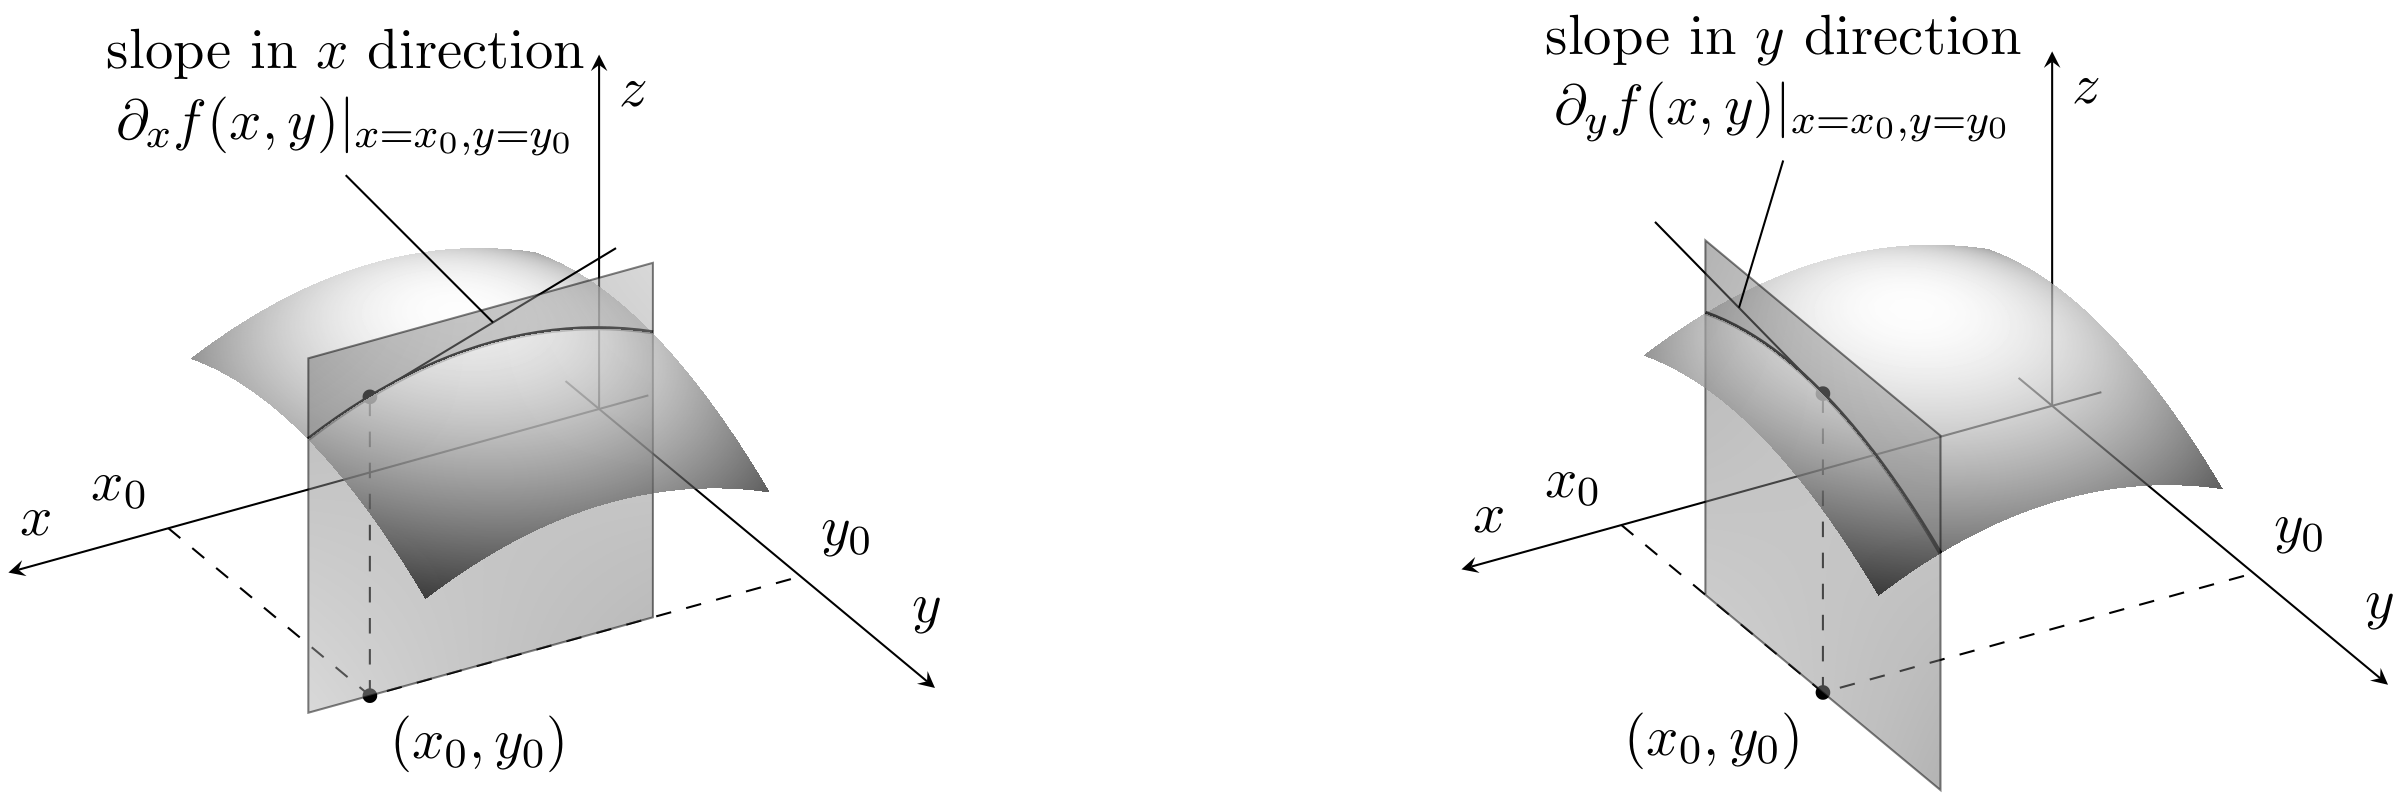
\includegraphics[width=0.9\textwidth]{derivate-parziali-significato-geometrico.png}
          \vspace{4mm}

          Questi due coefficienti angolari sono quelli delle rette tangenti al grafico che stanno sulla rispettiva traccia e che sono inoltre passanti per il punto \((x_0,y_0,f(x_0,y_0))\).

          Il piano formato dalle due rette rappresenta il piano tangente alla funzione nel punto \((x_0,y_0)\), ed ha equazione:

          \[
              z = f(x_0,y_0) + f_x(x_0,y_0) (x-x_0) + f_y(x_0,y_0) (y-y_0)
          \]
\end{itemize}

\subsubsection*{Esempio}

Scrivere l'equazione del piano tangente alla funzione \(z = x^{2}+y^{2}\) in \(P_0=(1,2)\),
dove \((x,y,z) \in S\), con \(S\) il grafico della funzione \(f(x,y)\).

Usando l'equazione del piano tangente:
\[
    P_0=(1,2) \iff (1,2,5) \in S
\]
\[
    z= 5+ 2(x-1) + 4(y-2) = 2x+4y -5
\]
quindi l'equazione richiesta è:
\[
    z = 2x+4y-5
\]

Vediamolo graficamente:
\filbreak{}

\begin{center}
    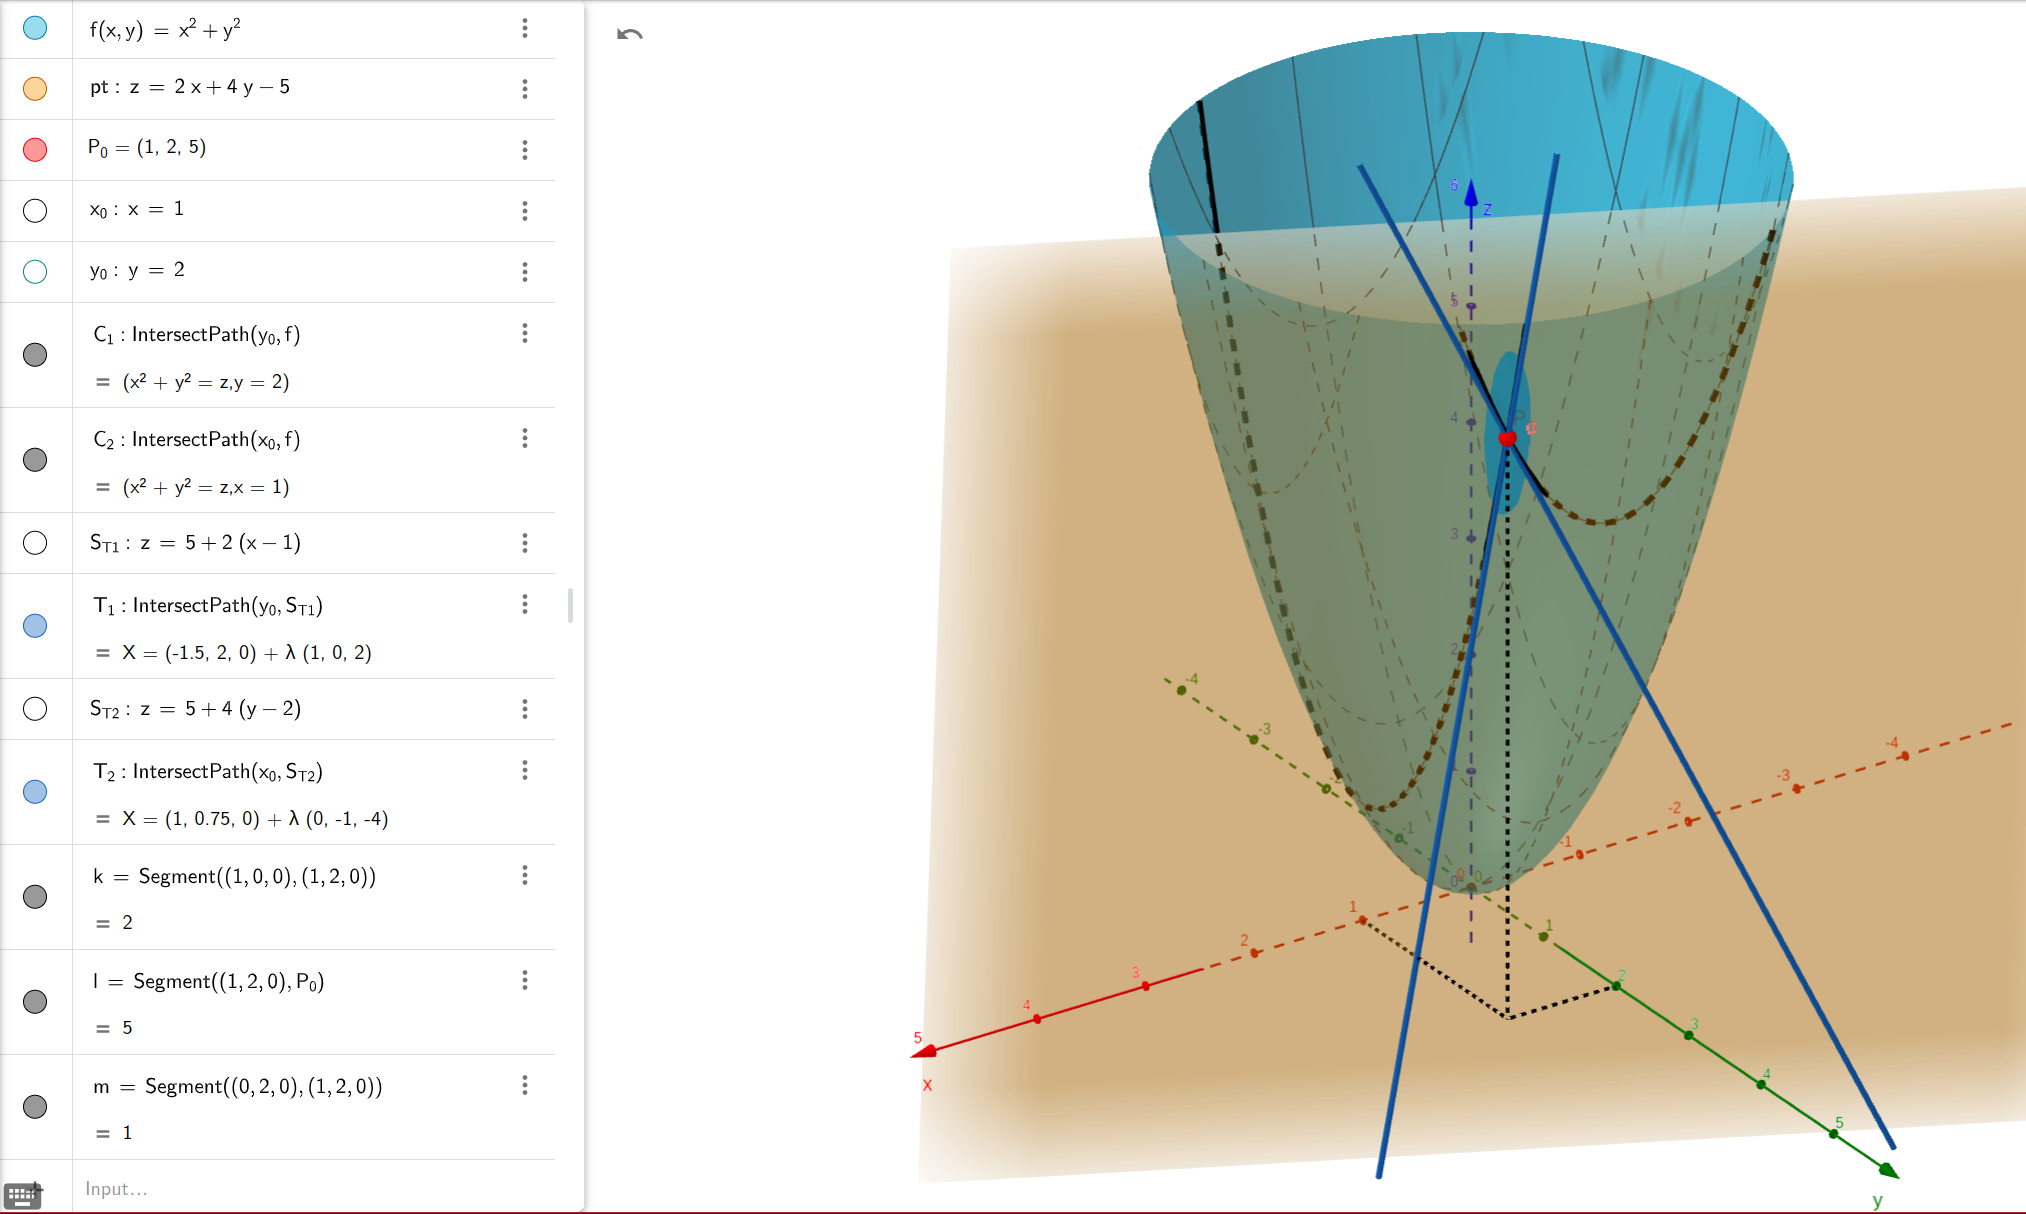
\includegraphics[width=0.79\textwidth]{piano-tangente-1.png}
    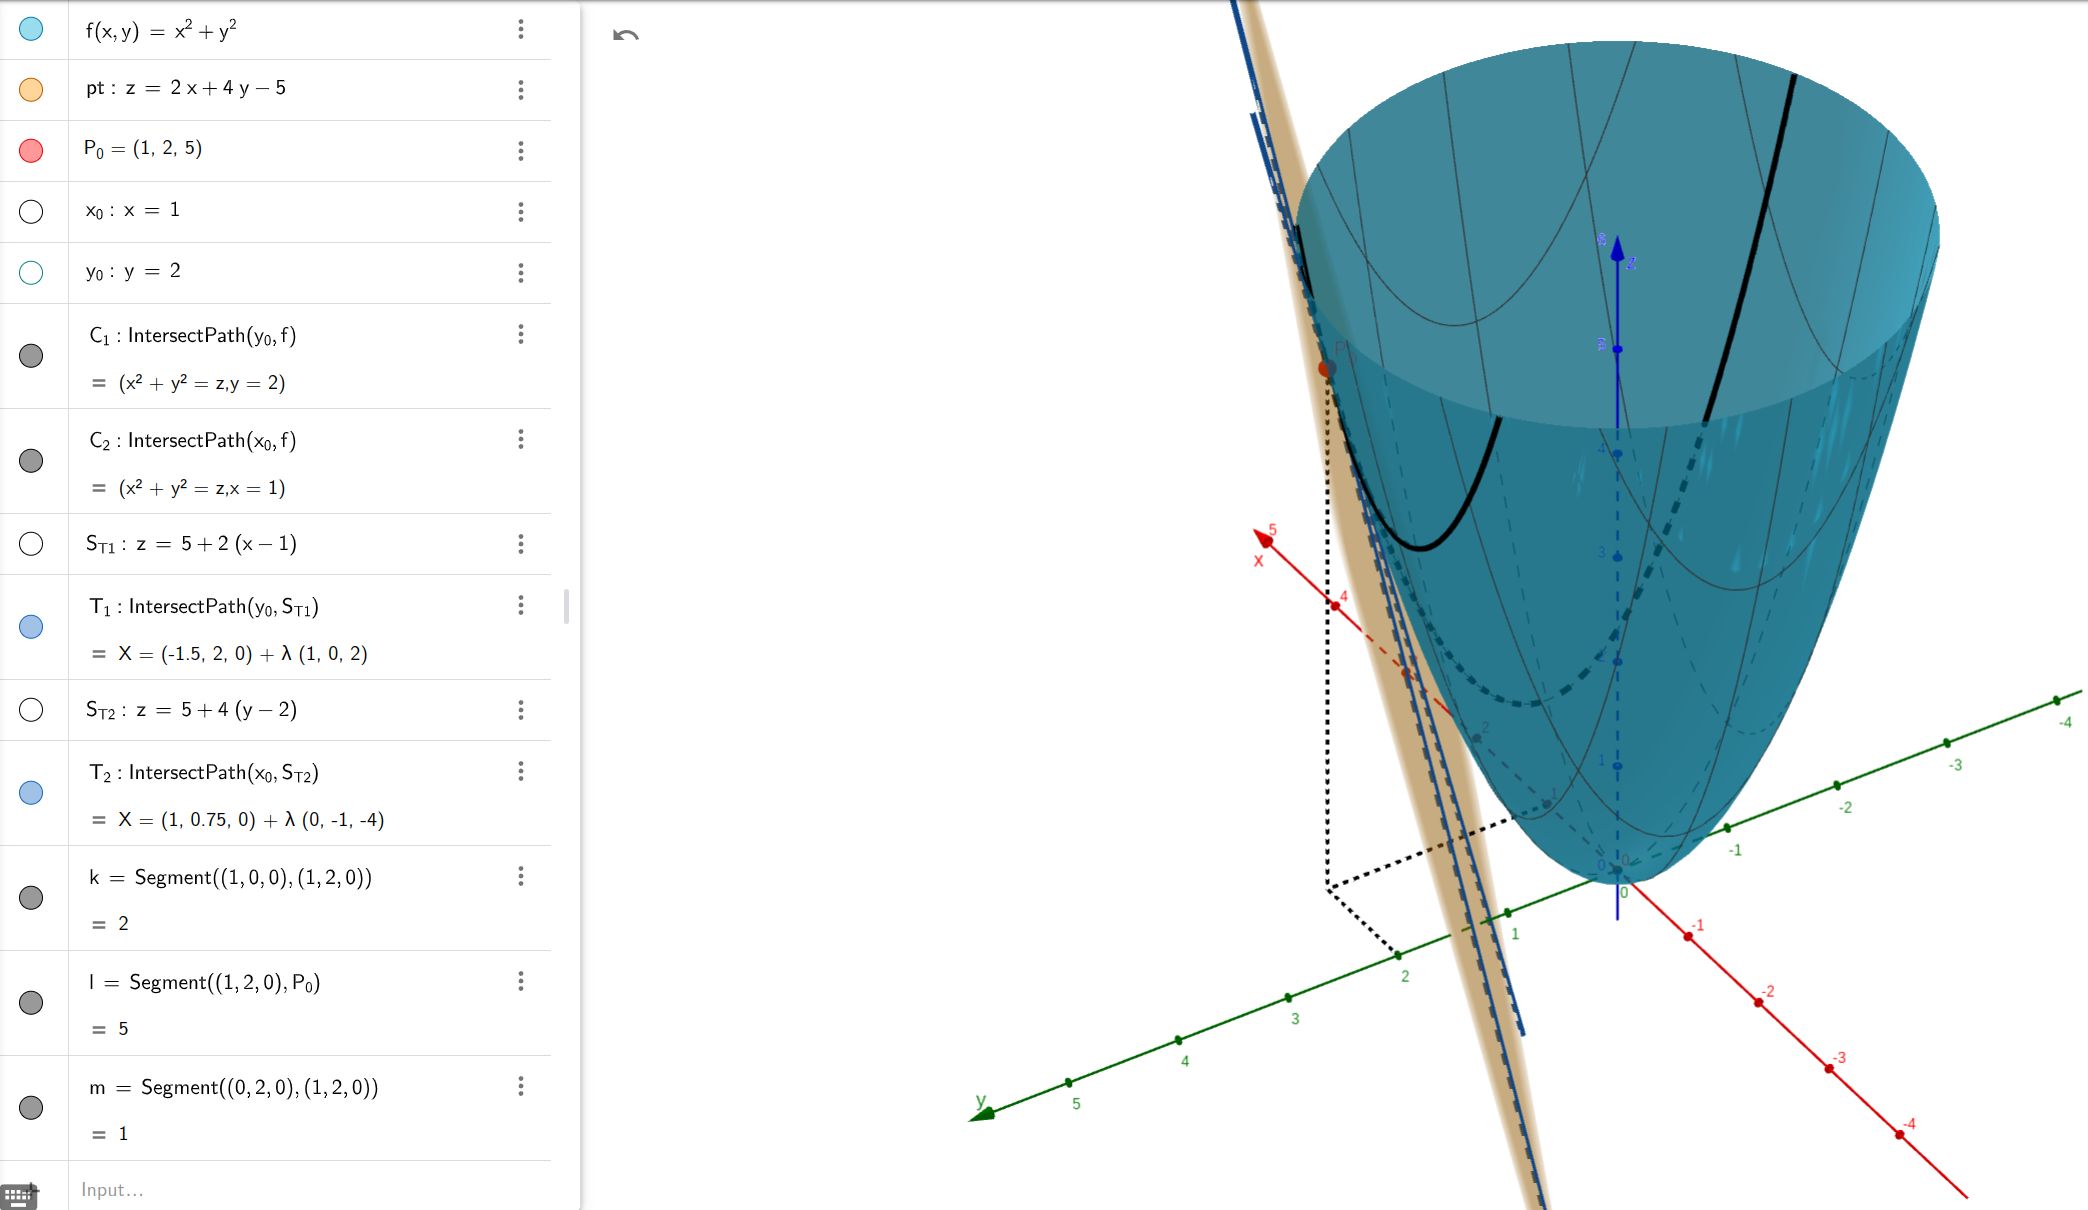
\includegraphics[width=0.79\textwidth]{piano-tangente-2.png}
    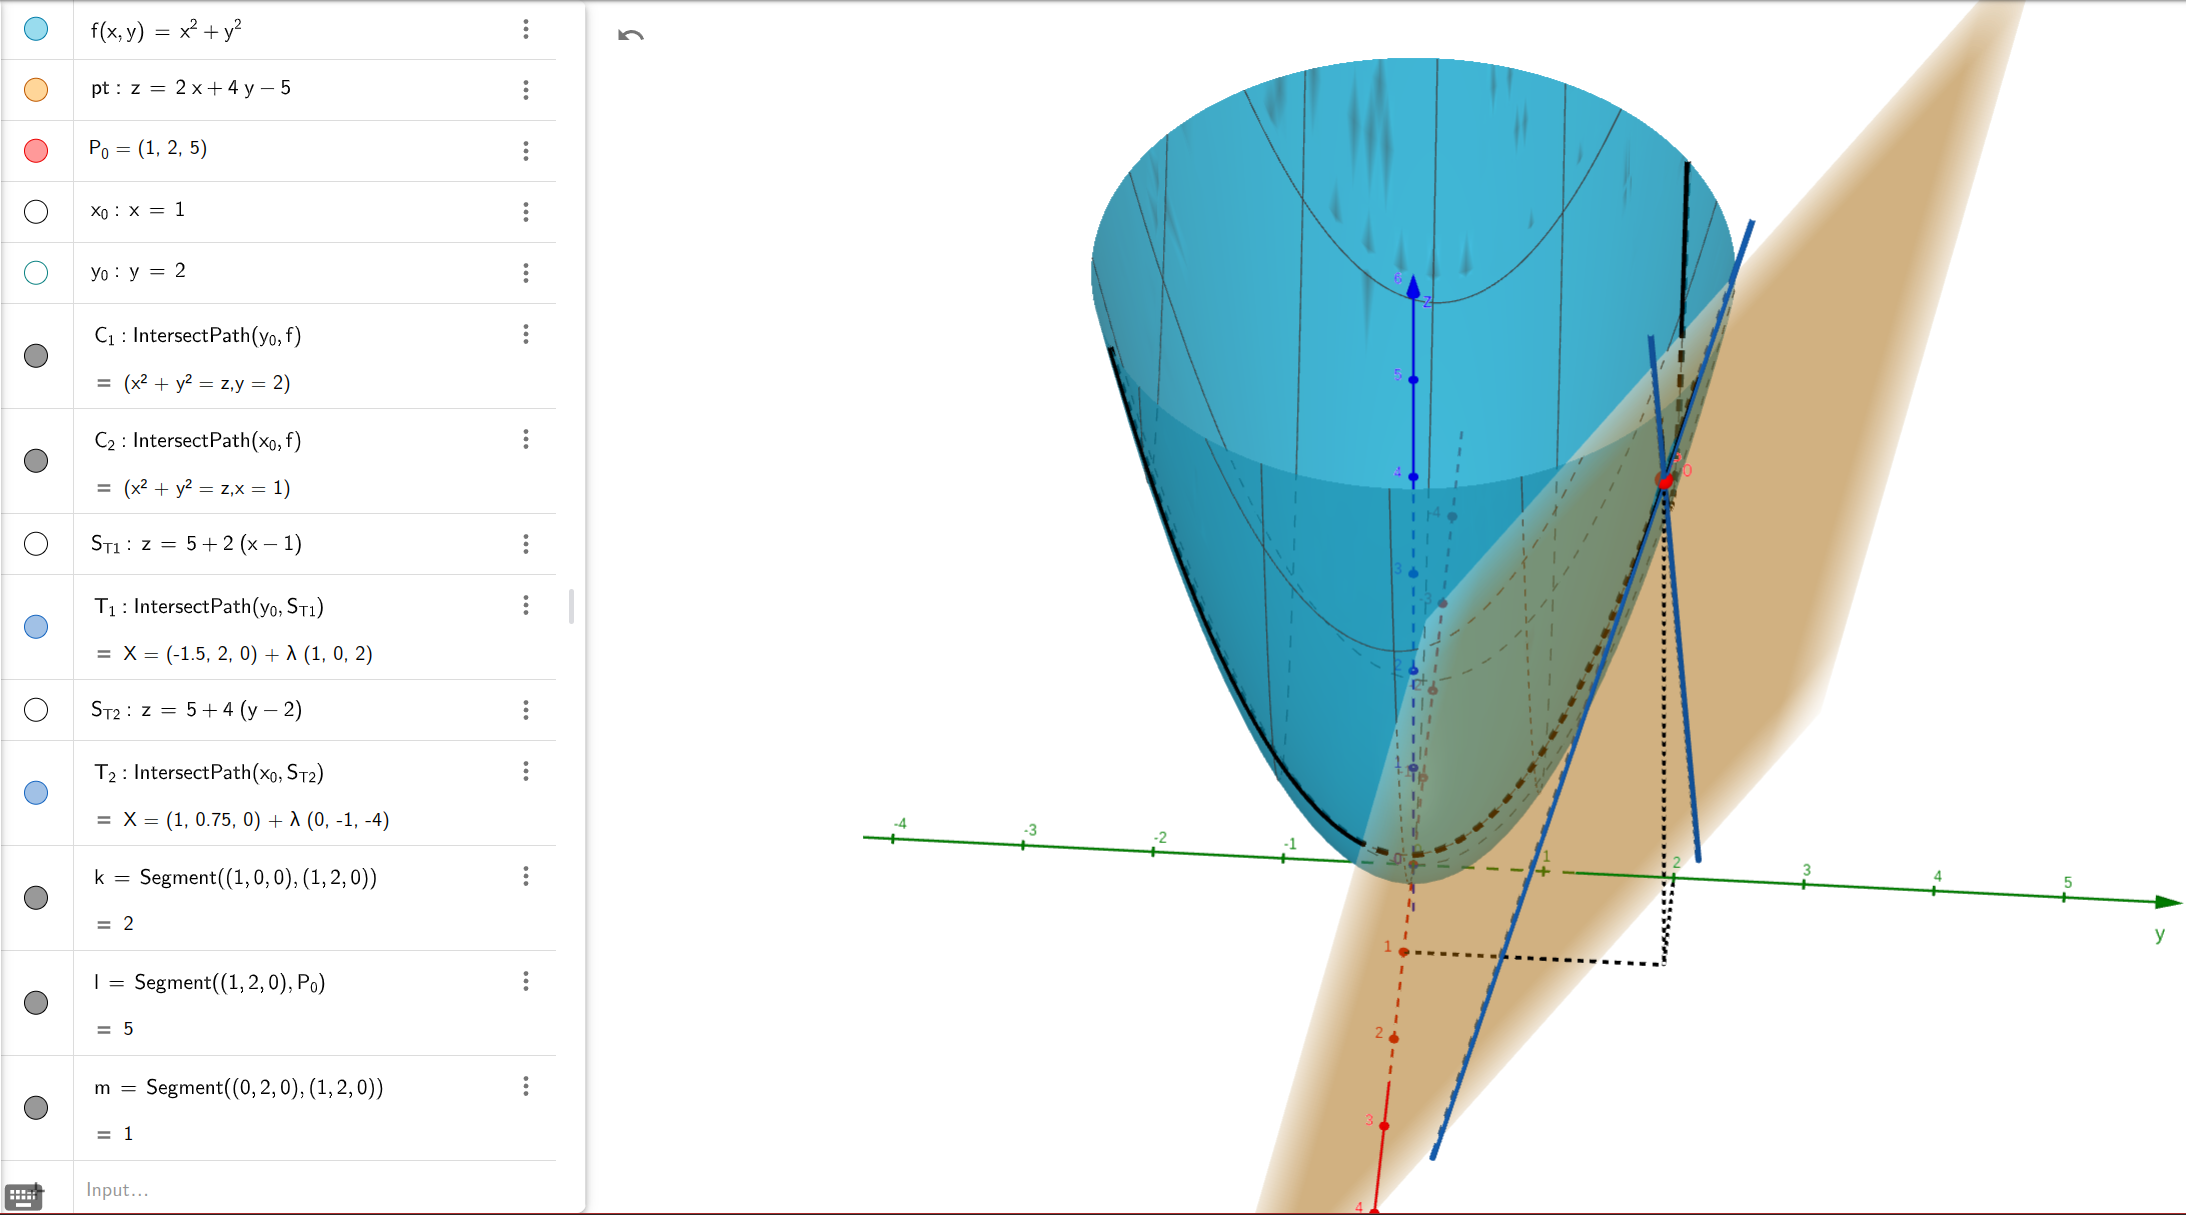
\includegraphics[width=0.79\textwidth]{piano-tangente-3.png}
\end{center}

\filbreak{}
\subsubsection{Definizione di derivabilità con il vettore gradiente}

Sia \(f: A \subseteq \R^2 \to \R \);

\(f\) si dice derivabile in \(A\) se esistono \(\frac{\partial f}{\partial x}\) e \(\frac{\partial f}{\partial y}\) in ogni punto di \(A\).

Ovvero, se esiste il \textbf{vettore gradiente}:

\[
    \nabla f(x,y)=\left( \frac{\partial f}{\partial x}(x,y), \frac{\partial f}{\partial y}(x,y) \right) \in \R^2
\]

Il vettore gradiente di \(f\) in \((x_0, y_0)\) è un vettore.

\textbf{In generale}:

In generale, per \(n\) variabili:

Data \(f: A \subseteq \R^n \to \R \), e \(\ux = (x_1, \ldots, x_n)\);

\(f\) è derivabile in \(\ux \in A\) se:

\[\exists \frac{\partial f}{\partial x_i}(\ux) ~\forall i = 1,\ldots,n\]

Ovvero se esiste finito il vettore gradiente:
\[
    \nabla f(\ux ) = \left( \frac{\partial f}{\partial x_1}\left(\ux\right), \frac{\partial f}{\partial x_2}\left(\ux\right), \ldots , \frac{\partial f}{\partial x_n}(\ux ) \right) \in \Rn
\]

\filbreak{}
\subsubsection{Derivata direzionale}

La derivata parziale è possibile scriverla anche secondo un'altra notazione. Partendo dalla notazione standard vista fino a ora:

\[
    f_{x_i} (\ux ) = \frac{\partial f}{\partial x_i}(\ux )
\]

definisco un \textbf{versore}, ovvero un vettore di modulo 1, nel modo seguente \(\forall i = 1, \ldots ,n\):

\[
    \underline{e_i} = (0, \ldots 0,1,0,\ldots,0)
\]

quindi, posso dire che la derivata parziale è data dal seguente limite, purché esista e sia finito:

\[
    \lim_{ h \to 0 } \frac{f(\ux + h \underline{e_i}) - f(\ux )}{h} = f_{x_i}(\ux )
\]

dove \(\ux + h \underline{e_i} = (x_1, \ldots, x_i, \ldots, x_n) + (0,\ldots,0,h,0,\ldots,0)\) è la \textbf{notazione vettoriale} di \(\ux \).

Dunque, espandendo:

\[
    f( \ux +h \underline{e_i} ) = f( x_{1}, \ldots , x_{i-1},x_{i}+h , x_{i+1}, \ldots ,x_{n})
\]

vediamo che dipende solo da h; quindi la derivata direzionale di \(f\) nella direzione di \(\underline{e_i}\) è la derivata della funzione di 1 variabile:

\[
    g(h) = f(\ux + h \underline{e_i} )
\]

Se g è derivabile in \(h=0\), allora:

\[
    g'(0) = \frac{\partial f}{\partial x_i}(\ux ) = f_{x_i}(\ux)
\]

ovvero significa che esiste, finito, il limite:

\[
    g'(0) = \lim_{ h \to 0 } \frac{g(h) - g(0)}{h-0} = \lim_{ h \to 0 } \frac{f(\ux +h \underline{e_i} ) - f(\ux )}{h} = \frac{\partial f}{\partial x_i}(\ux)
\]

\subsubsection*{Generalizzazione}

Se abbiamo \(\vec{v} \), una direzione in \(\Rn \) di modulo 1, ovvero \(\vec{v}\) versore in \(\Rn \):

\[
    \norm{\vec{v}} = \sqrt{\sum^{n}_{i=1} {v_i}^{2}} = 1
\]

Allora, definisco la \textbf{derivata direzionale} come:

\[
    \frac{\partial f}{\partial \vec{v}}(\ux) = D_{\vec{v}} f(\ux ) = \lim_{ h \to 0 } \frac{f(\ux +h \vec{v} ) -f(\ux )}{h}
\]

\filbreak{}
\subsubsection*{Per n=2}

Se prendiamo un punto \(P_0 = (x_0, y_0)\), le due derivate direzionali saranno:
\begin{align*}
    \frac{\partial f}{\partial x}(P_0) = \text{derivata parziale di f nella direzione di } e_1 = \text{asse } x \\[3mm]
    \frac{\partial f}{\partial y}(P_0) = \text{derivata parziale di f nella direzione di } e_2 = \text{asse } y
\end{align*}

\subsubsection*{Per n=3}

Sia \(f: A \subseteq \R^{3} \rightarrow \R \) una funzione;

Consideriamo \(\vec{v} = (a,b,c) \in \R^{3}\) come vettore direzionale. Vale quindi \(\norm{\vec{v}} =1\).

Calcoliamo la derivata direzionale rispetto a \(\vec{v}\), che è il seguente limite, se esiste, finito:

\[
    D_{\vec{v}} f(\ux ) = \lim_{ h \to 0 } \frac{f(\ux + h \vec{v} ) -f(\ux )}{h}
\]

dove \(\ux = (x_0,y_0,z_0)\), quindi:

\[
    D_{\vec{v}} f(\ux ) = \lim_{ h \to 0 } \frac{f(x_0+ha,y_0+hb,z_0+hc) - f(x_0,y_0,z_0)}{h}
\]

Quindi, se il limite esiste ed è finito, avremmo le 3 derivate parziali:
\begin{align*}
    \frac{\partial f}{\partial x}(\underline{P_0}) = f_x(\underline{P_0}) = D_{\vec{e_1}}f(\underline{P_0}) = \text{derivata parziale di f nella direzione di } \vec{e}_1 \\[3mm]
    \frac{\partial f}{\partial y}(\underline{P_0}) = f_y(\underline{P_0}) = D_{\vec{e_2}}f(\underline{P_0}) = \text{derivata parziale di f nella direzione di } \vec{e}_2 \\[3mm]
    \frac{\partial f}{\partial z}(\underline{P_0}) = f_z(\underline{P_0}) = D_{\vec{e_3}}f(\underline{P_0}) = \text{derivata parziale di f nella direzione di } \vec{e}_3
\end{align*}

dove, \(\vec{e}_1, \vec{e}_2, \vec{e}_3\) sono i versori degli assi \(x,y,z\), ovvero:
\begin{align*}
     & \vec{e}_1 = (1,0,0) = \vec{i} \\
     & \vec{e}_2 = (0,1,0) = \vec{j} \\
     & \vec{e}_3 = (0,0,1) = \vec{w}
\end{align*}

\subsubsection*{Conclusione}

Per concludere, dire che \(f\) è derivabile in \(P_0 \in \Rn \) equivale a dire che esiste il vettore gradiente:

\[
    \Rn \ni \nabla f(\ux) = \left( \frac{\partial f}{\partial x_1}(\ux), \ldots, \frac{\partial f}{\partial x_n}(\ux) \right)
\]

con \(x_i\) tutte le varie direzioni.

\newpage
\subsection{Differenziabilità}

\subsubsection{Differenza tra derivabilità e differenziabilità}

Il fatto che la funzione a \textbf{una variabile} sia derivabile in un punto mi dice che esiste la retta tangente in quel punto.

Per le funzioni a due variabili questo non è vero, infatti, per le funzioni a più di una variabile:
\[\text{derivabilità} \ne \text{differenziabilita}\]

Questo è dato dal fatto che per le funzioni in due variabili la derivabilità non implica la continuità:

\[
    derivabile \centernot\implies continua
\]

\textbf{Controesempio}

Calcolare, se esistono, le derivate parziali in \((0,0)\):

\[
    f(x,y)=
    \begin{cases}
        \frac{xy^{2}}{x^{2}+y^{4}} & \text{se}\ (x,y)\neq (0,0) \\
        0                          & \text{se}\ (x,y)=(0,0)
    \end{cases}
\]

Consideriamo le tracce:

\[
    f(x,0) = 0 \quad;\quad f(0,y) =0
\]

Dunque ottengo due funzioni identicamente nulle che sono derivabili con derivata nulla:

\[
    f_x(0,0) = f_y(0,0) = 0
\]

Osserviamo però che in \((0,0)\) la funzione non è continua perché:

\[
    \lim_{ (x,y) \to (0,0) } \frac{xy^{2}}{x^{2}+y^{4}} \text{ non esiste}
\]

Per risolvere questo problema, quello che ci servirà sarà il concetto di \textbf{differenziabilità}.

\filbreak{}
\subsubsection{Definizione di differenziabilità}

Avendo una funzione \(f:A\subseteq \Rn \rightarrow \R \) con \(A\) aperto

f è derivabile in \(\ux =(x_1, \ldots ,x_n) \in A\) equivale a dire che esiste il vettore gradiente:

\[
    \nabla f(\ux ) = \left( \frac{\partial f}{\partial x_1}(\ux ), \ldots , \frac{\partial f}{\partial x_n}(\ux ) \right)
\]

\defn{Differenziabilità}{
Il concetto di differenziabilità è più forte rispetto al concetto di derivabilità.

Infatti, si dice che \(f\) è differenziabile in \(\ux \in A \) se \(f\) è derivabile in \(\ux \) e inoltre vale la seguente relazione:

\[
    \lim_{ \uh \to 0 } \frac{f( \ux + \uh ) - f( \ux ) - \langle \nabla f(\ux ), \uh \rangle}{\norm{\uh}} =0
\]

dove \(\uh \in \Rn \); e inoltre ricordo che:

\[
    \norm{\uh} = \sqrt{\sum^{n}_{i=1} h_i^{2}}
\]

\[
    \langle \nabla f(\ux ), \uh \rangle = \frac{\partial f}{\partial x_1}(\ux )\cdot h_1+ \frac{\partial f}{\partial x_2}(\ux ) \cdot h_2+ \cdots  + \frac{\partial f}{\partial x_n}(\ux ) \cdot h_n
\]

Se \(f\) è differenziabile in ogni punto di \(A\) si dice che \(f\) è differenziabile in \(A\)
}

Da notare che il prodotto scalare \(\langle \nabla f(\ux ), \uh \rangle \) rappresenta l'incremento che io faccio verso ogni direzione per poter ``vedere'' che cosa succede quando mi sposto un ``pochino'' in ogni direzione.

\defn{Differenziale}{
    Definisco come \(L : \Rn \rightarrow \R \) l'applicazione che ad \(\uh \) associa il prodotto scalare:

    \[
        \uh \mapsto \langle \nabla f(\ux ) , \uh \rangle
    \]

    Questa applicazione si chiama \textbf{differenziale} di \(f\) in \(\ux \) e si indica con \(\diff f(\ux)\)

    Questa è un'\textbf{applicazione lineare} da \(\Rn \) in \(\R \) della variabile \(\uh \)

    \[
        \diff f(\ux ) (\uh ) = \langle \nabla f(\ux ) , \uh \rangle
    \]
}

\filbreak{}
Usando questa nomenclatura, possiamo dunque dire che \(f\) è differenziabile in \(\ux \in A\) se esiste un \textbf{funzionale lineare} \(L: \Rn \rightarrow \R \) tale che:

\[
    \lim_{ \uh \to 0 } \frac{f(\ux+\uh) -f(\ux) - L(\uh)}{\norm{\uh}} = 0
\]

In \(\Rn \) ogni funzionale lineare si rappresenta come un opportuno prodotto scalare.


Se \(L: \Rn \rightarrow \R \) è lineare allora esiste \(\underline{l} \in \Rn \) tale che:

\[
    L(\uh ) = \langle \uh , \underline{l} \rangle \quad \forall \uh \in \Rn
\]

Dunque, \(f: A \subseteq \Rn \rightarrow \R \) è differenziabile in \(\ux \in A\) se è derivabile in \(\ux \) e se:

\[
    f(\ux + \uh ) \xrightarrow[\uh \to 0]{} f(\ux ) + \langle \nabla f(\ux ), \uh \rangle + o(\norm{\uh})
\]

\subsubsection{Significato geometrico del differenziale}

La differenziabilità è legata all'esistenza del piano tangente al grafico della \(f: A \subseteq \Rn \to \R \) in un punto \(\ux_0\).

Supponiamo che \(f\) sia differenziabile in \(\ux_0 \in A \), allora, tornando alla relazione definita dalla differenziabilità, per \(\uh \to 0\):

\[
    f(\ux_0+\uh) = f(\ux_0) +\langle \nabla f(\ux_0) , \uh \rangle  + o(\norm{\uh} )
\]

riscrivendolo per \(\uh = \ux - \ux_0\):

\[
    f(\ux) = \underbrace{f(\ux_0)}_{\begin{smallmatrix}\text{punto di} \\ \text{partenza}\end{smallmatrix}} + \underbrace{\langle \nabla f(\ux_0), \ux-\ux_0 \rangle}_\text{il mio spostamento} + \underbrace{o(\norm{\ux-\ux_0})}_{\begin{smallmatrix}\text{l'errore commesso} \\ \text{spostandosi}\end{smallmatrix}}
\]

e dunque la funzione lineare che associa:
\[\ux \mapsto  f(\ux_0 ) + \langle \nabla f(\ux_0 ), \ux-\ux_0 \rangle \]
ci fornisce un'\textbf{approssimazione di tipo lineare} della \(f(\ux)\) nel punto \(\ux_0\) a meno di infinitesimi di ordine superiore alla distanza euclidea tra \(\ux \) e \(\ux_0\):

\[
    d(\ux,\ux_0) = \norm{\ux-\ux_0}
\]

\textbf{Importante}:

Il grafico di questa funzione lineare rappresenta il piano tangente al grafico di \(f\) nel punto \(\ux_0\) in cui la \(f\) è differenziabile.

Per \(n=2\) ritroviamo infatti l'equazione vista in precedenza del piano tangente al punto \(\ux_0\).

Questo è chiaro in due variabili perché ci spostiamo sia lungo le \(x\) che le \(y\) e quindi disegniamo un piano.

\pagebreak
\subsubsection{Differenziale come approssimazione lineare (per n=2)}

Consideriamo:

\[
    \underline{P_0} = (x_0,y_0)
\]

con \(f\) differenziabile in \(\underline{P_0}\).

L'equazione del piano tangente al grafico di \(f\) nel punto \(\underline{P_0}\) è:

\[
    z= f(\underline{P_0}) + \langle \nabla f(\underline{P_0}), \underline{P}-\underline{P_0} \rangle
\]

ovvero, sapendo che:

\[
    \nabla f(\underline{P_0}) = \left( \frac{\partial f}{\partial x}(x_0,y_0), \frac{\partial f}{\partial y}(x_0,y_0) \right)
\]

allora l'equazione del piano tangente nel punto (\(x_0,y_0,f(x_0,y_0)\)) diventa:

\[
    z = f(x_0,y_0) + \frac{\partial f}{\partial x}(x_0,y_0) (x-x_0) + \frac{\partial f}{\partial y}(x_0,y_0) (y-y_0)
\]

Scriviamo la definizione di differenziale in \(\uh=(h_x,h_y)\) per \((h_x,h_y) \rightarrow (0,0)\):

\[
    f(x_0+h_x,y_0+h_y) = f(x_0,y_0) + \frac{\partial f}{\partial x}(x_0,y_0) \cdot h_x + \frac{\partial f}{\partial y}(x_0,y_0) \cdot h_y + \underbrace{ o\left( \sqrt{h_x^{2}+h_y^{2}} \right)}_{o(\norm{\uh})}
\]
\begin{equation*}
    \text{e se pongo }
    \begin{cases}
        x_0 + h_x = x \\
        y_0 + h_y = y
    \end{cases}
    \implies \text{allora:}
\end{equation*}

\[
    f(x,y) = f(x_0,y_0) + \frac{\partial f}{\partial x}(x_0,y_0) (x-x_0) + \frac{\partial f}{\partial y}(x_0,y_0) (y-y_0) + \underbrace{o\left( \sqrt{{(x-x_0)}^{2}+{(y-y_0)}^{2}} \right)}_\text{\(d(\underline{P},\underline{P}_0)\)}
\]

E dunque, per le funzioni differenziabili si ha che il piano di equazione:

\[
    z= f(x_0,y_0) + \frac{\partial f}{\partial x}(x_0,y_0)(x-x_0) + \frac{\partial f}{\partial y}(x_0,y_0) (y-y_0)
\]

dista dal grafico di \(f\) per una quantità che va a zero più rapidamente di quanto \(\underline{P}\) si avvicini a \(\underline{P}_0\).

\[
    f(x,y) - \left[ f(x_0,y_0) + \frac{\partial f}{\partial x}(x_0,y_0) (x-x_0) + \frac{\partial f}{\partial y}(x_0,y_0) (y-y_0) \right] = \underbrace{o\left( \sqrt{{(x-x_0)}^{2}+{(y-y_0)}^{2}} \right)}_\text{\(d(\underline{P},\underline{P}_0)\)}
\]

\filbreak{}
quindi:

\[
    \lim_{ (x,y) \to (x_0,y_0) } \frac{f(x,y) - \left[ f(x_0,y_0) + \frac{\partial f}{\partial x}(x_0,y_0) (x-x_0) + \frac{\partial f}{\partial y}(x_0,y_0) (y-y_0) \right] }{\sqrt{{(x-x_0)}^{2}+{(y-y_0)}^{2}}}= 0
\]

La funzione \(L: \R^{2} \rightarrow \R \):

\[
    L(x,y) = f(x_0,y_0) + \frac{\partial f}{\partial x}(x_0,y_0) (x-x_0) + \frac{\partial f}{\partial y}(x_0,y_0) (y-y_0)
\]

il cui grafico è il piano tangente al grafico di \(f\) in \((x_0,y_0)\), si chiama anche \textbf{linearizzazione} di \(f(x,y)\) in \((x_0,y_0)\).

L'applicazione delle \(f\) mediante tale piano viene detta \textbf{approssimazione lineare} della \(f\) in \((x_0,y_0)\)

\pagebreak
\subsubsection{Esempio di esercizio sulla differenziabilità}

Data la funzione:

\[
    f(x,y) = \begin{cases}
        \displaystyle \frac{x^{3}+2y^{4}}{x^{2}+y^{2}} & \text{se \((x,y) \neq (0,0)\)} \\
        0                                              & \text{se \((x,y) = (0,0)\)}
    \end{cases}
\]

\begin{enumerate}
    \item Stabilire in quali punti del piano è derivabile, calcolandone le derivate in tale caso
    \item Stabilire in quali punti del piano è differenziabile
    \item Stabilire il più grande aperto \(A \subseteq \R^{2}\) su cui \(f\) è \(C^{1}\)
\end{enumerate}

\textbf{Soluzione}

\begin{enumerate}
    \item Osserviamo che se \((x,y) \neq (0,0)\) non presenta problemi ed è sempre derivabile in quanto composizione di funzioni sempre derivabili (polinomi). Le sue derivate parziali sono:

          \begin{align*}
               & \frac{\partial f}{\partial x}(x,y) = \frac{3x^{2}(x^{2}+y^{2})-2x(x^{3}+2y^{4})}{{(x^{2}+y^{2})}^{2}}= \frac{x^{4}+3x^{2}y^{2}-4xy^{4}}{{(x^{2}+y^{2})}^{2}}     \\[3mm]
               & \frac{\partial f}{\partial y}(x,y) = \frac{8y^{3}(x^{2}+y^{2}) - 2y(x^{3}+2y^{4})}{{(x^{2}+y^{2})}^{2}} = \frac{4y^{5}+8x^{2}y^{3}-2x^{3}y}{{(x^{2}+y^{2})}^{2}}
          \end{align*}

          Controlliamo ora la derivabilità in \((0,0)\):

          \[
              f(0,y) = 2y^{2} \implies f_y(0,y) = 4y \implies f_y(0,0) = 0
          \]
          \[
              f(x,0) = x \implies f_x(x,0) = 1 \implies f_x(0,0) = 1
          \]

          Dunque è derivabile anche in \((0,0)\) e di conseguenza in tutto \(\R^2\).

    \item Bisogna vedere che cosa succede in \((0,0)\) che è l'unico punto problematico per la continuità di \(f(x,y)\).

          Per essere differenziabile in \((0,0)\) deve essere:

          \[
              f(x,y) - f(0,0) - \frac{\partial f}{\partial x}(0,0) (x-0) - \frac{\partial f}{\partial y}(0,0) (y-0) = o\left( \sqrt{x^{2}+y^{2}} \right)
          \]

          e quindi deve valere il seguente limite:

          \begin{align*}
              \lim_{ (x,y) \to (0,0) } \frac{ \frac{x^{3}+2y^{4}}{x^{2}+y^{2}}-0 -1(x-0) -0(y-0)}{\sqrt{x^{2}+y^{2}}}
               & = \lim_{ (x,y) \to (0,0) } \frac{x^3+2y^{4}-x(x^2+y^2)}{(x^{2}+y^{2}) {(x^{2}+y^{2})}^{ \frac{1}{2}}} \\
               & = \lim_{ (x,y) \to (0,0) } \frac{2y^{4}-xy^{2}}{{(x^{2}+y^{2})}^{ \frac{3}{2}}}
              = 0
          \end{align*}

          Noto che:

          \[
              \left|\frac{2y^{4}-xy^{2}}{{(x^{2}+y^{2})}^{ \frac{3}{2}}}\right| \le \left|\frac{2y^{4}}{{(x^{2}+y^{2})}^{ \frac{3}{2}}}\right| \le \left|2y^{4}\right| = 2y^4 \xrightarrow[(x,y) \to (0,0)]{} 0
          \]

          Quindi per il teorema del confronto abbiamo verificato che vale il limite, e che quindi la funzione è differenziabile anche in \((0,0)\).
    \item Tutto \(\R^2\)
\end{enumerate}

\pagebreak
\subsubsection{Definizione formale di differenziabilità}

\defn{Differenziabilità}{
    Sia \(f:A \subseteq \Rn \rightarrow \R \) una funzione, con \(A\) aperto, e sia \(\ux_0 \in A\).

    Si dice che \(f\) è differenziabile in \(\ux_0\) se \(\exists L:\Rn \rightarrow \R \) funzione lineare tangente a \(f\)  in \(\ux_0\) tale che:

    \[
        \lim_{ \uh \to 0 } \frac{f(\ux_0+\uh) - f(\ux_0) -L(\uh)}{\norm{\uh}} = 0
    \]

    dove \(L(\uh) = \langle \nabla f(\ux_0), \uh \rangle \)
}

\subsubsection{Teoremi sulla differenziabilità e continuità}

\teorema{}{
    Sia \(f: A \subseteq \Rn \to \R \); Sia inoltre \(\ux_0 \in A\);

    \(f\) è differenziabile in \(\ux_0 \implies f\) è continua in \(\ux_0 \)
}


\begin{proof}
    Per dimostrare che \(f\) è continua in \(\ux_0 \) devo far vedere che:

    \[
        \lim_{ \uh \to 0 } f(\ux_0 + \uh) = f( \ux_0 )
    \]

    \[
        \lim_{ \uh \to 0 } f(\ux_0 + \uh ) \overset{\text{differenziabile}}{=}
        \lim_{ \uh \to 0 } \left[ f(\ux_0) + \langle \nabla f(\ux_0), \uh \rangle + o(\norm{\uh}) \right]
    \]

    applichiamo la disuguaglianza di Cauchy-Schwarz:

    \[
        \langle \nabla f(\ux_0), \uh \rangle \le
        \Big|\langle \nabla f(\ux_0), \uh \rangle\Big| \le
        \norm{\nabla f(\ux_0)} \cdot \norm{\uh}
        \xrightarrow[\uh \to 0]{} 0
    \]

    quindi abbiamo che:

    \[
        \lim_{ \uh \to 0 } \left[ f(\ux_0) + \underbrace{\langle \nabla f(\ux_0),\uh \rangle}_\text{\(\rightarrow 0\)} + \underbrace{o(\norm{\uh})}_\text{\(\rightarrow 0\)} \right] = f(\ux_0)
    \]
\end{proof}

\pagebreak
\teorema{Teorema del differenziale totale}{
    Sia la funzione \(f: A \subseteq \Rn \rightarrow \R \) derivabile in \(A\) con \(A\) aperto.

    Se le derivate parziali \(f_{x_1}, \ldots, f_{x_n}\) sono continue in \(\ux_0 \in A\) allora \(f\) è differenziabile in \(\ux_0 \)
}

\begin{proof}
    Per \(n=2\)

    Sia \(f = f(x,y)\) con \((x,y) \in A \subseteq \R^{2}\), e sia \(\uh = (h,k)\):
    \begin{align*}
        f(x+h,y+k) - f(x,y) & = f(x+h,y+k) + f(x,y+k) - f(x,y+k) - f(x,y)                                                                        \\
                            & = \underbrace{[f(x+h,y+k) - f(x,y+k) ]}_{f(b,y+k) - f(a,y+k)} + \underbrace{[f(x,y+k) - f(x,y)]}_{f(x,b) - f(x,a)}
    \end{align*}

    Applico il teorema di Lagrange sulle due quadre, per cui:
    \begin{align*}
        \exists x_0 & \in (x,x+h) \giventhat f(x+h,y+k)-f(x,y+k) = \frac{\partial f}{\partial x}(x_0,y+k) \cdot [(x+h)-(x)] \\
        \exists y_0 & \in (y,y+k) \giventhat f(x,y+k)-f(x,y) = \frac{\partial f}{\partial y}(x,y_0) \cdot [(y+k)-(y)]
    \end{align*}
    Dunque:
    \begin{align*}
        f(x+h,y+k) - f(x,y) & = \frac{\partial f}{\partial x}(x_0,y+k) (x +h -x) + \frac{\partial f}{\partial y}(x,y_0) ( y + k -y) \\
                            & = \frac{\partial f}{\partial x}(x_0,y+k) h + \frac{\partial f}{\partial y}(x,y_0)k
    \end{align*}
    Ora, parto dalla definizione di differenziabilità per \(f\) in \((x+h,y+k)\) e sostituisco quanto ottenuto sopra:

    \[
        \frac{f(x+h,y+k) - f(x,y) - f_x(x,y)h - f_y(x,y) k}{\sqrt{h^{2}+k^{2}}} =
    \]

    \[
        = \frac{\left[ f_x(x_0,y+k) h + f_y(x,y_0) k \right] -f_x(x,y)h -f_y(x,y)k}{\sqrt{h^{2}+k^{2}}} =
    \]

    \[
        = \frac{[f_x(x_0,y+k) - f_x(x,y)] h + [f_y(x,y_0) - f_y(x,y)] k}{\sqrt{h^{2}+k^{2}}}
    \]

    metto tutto in valore assoluto e maggioro:
    \begin{align*}
        [\ldots] & \le \left|\frac{[f_x(x_0,y+k) - f_x(x,y)] h + [f_y(x,y_0) - f_y(x,y)] k}{\sqrt{h^{2}+k^{2}}}\right|                    \\
                 & \le |f_x(x_0,y+k) - f_x(x,y)| \frac{|h|}{\sqrt{h^{2}+k^{2}}} + | f_y(x,y_0) - f_y(x,y)| \frac{|k|}{\sqrt{h^{2}+k^{2}}} \\
                 & \le |f_x(x_0,y+k) - f_x(x,y)| + |f_y(x,y_0) - f_y(x,y)|
    \end{align*}

    \filbreak{}
    Quando \((h,k) \rightarrow (0,0)\) succede che \((x_0,y_0) \rightarrow (x,y)\). Inoltre, essendo \(f_x\) e \(f_y\) continue in \((x,y)\):

    \[
        |\underbrace{f_x(x,y+k) - f_x(x,y)}_\text{\(\rightarrow 0\)}| + |\underbrace{f_y(x,y) - f_y(x,y)}_\text{\(\rightarrow 0\)}| \xrightarrow[\uh \to 0]{} 0
    \]

    Quindi \(f(\ux,\uy)\) è differenziabile in \(\ux_0\).

\end{proof}

\defn{Continuità di funzioni in più variabili}{
    Quindi una funzione \(f: A \subseteq \Rn \rightarrow \R \) continua in \(A\), si dice di classe \(C^{0}\) e si scrive \(f \in C^{0}(A)\)

    Se la funzione è derivabile in \(A\) e se le derivate parziali sono continue in \(A\) si dice che è di classe \(C^{1}\) su \(A\) e si scrive \(f \in C^{1}(A)\).

    \;

    In generale \(f \in C^{k}(A), k \in \N \) se \(f\) è derivabile fino all'ordine k, con tutte le derivate fino all'ordine k continue.

    \;

    Attenzione: Se la funzione \(f\) è solamente derivabile due volte su \(A\), questo non equivale a dire che \(f \in C^{2}(A)\)
}

\pagebreak
\subsubsection{Funzioni composte}

Interpretiamo il significato di quanto detto fino a ora usando le curve.

Vediamo un introduzione al seguente teorema fondamentale. In seguito vedremo la sua definizione formale con generalizzazione e dimostrazione.

\teorema{Regola della catena}{

Sia \(g : [-1,1] \rightarrow A\subseteq \Rn \) una curva continua;

Sia \(g(t)\) derivabile:
\begin{align*}
     & g(t) = (g_1(t),\ldots,g_n(t) ) \in \Rn \\[3mm]
     & g'(t) = (g_1'(t),\ldots,g_n'(t))
\end{align*}
Supponiamo inoltre che la curva passi per \(\ux_0\), ovvero che \(g(0) = \ux_0 \in A\), \(g'(0) = \vec{v} \in \Rn \).

Allora, se \(f: A \rightarrow \R \) è un'altra funzione differenziabile in \(\ux_0\), la funzione composta:
\[F: [-1,1] \to \R \]
\[t \mapsto F(t) = (f \circ g) (t) = f(g(t))\]
è differenziabile in \(0\).

Inoltre, si ha che:
\[
    F'(0) = \frac{\partial F}{\partial t} (0) = \frac{\partial (f \circ g)}{\partial t}(0) = \langle \nabla f(\ux_0), \underbrace{g'(0)}_\text{direzione \(\vec{v} \)} \rangle
\]

Questo si chiama \textbf{teorema delle derivate di funzioni composte} o regola della catena.

}

In sostanza questa regola ci dà una formula per la derivata direzionale, che può essere calcolata come:

\[
    \frac{\partial f}{\partial \vec{v}} (\ux_0) = \langle \nabla f(\ux_0), \vec{v} \rangle
\]

Dunque, la crescita di \(f\) in \(\ux_0\) lungo una qualsiasi curva \(g \) regolare (\(g \in C^{1}\)) uscente da \(\ux_0\) con velocità \(g'(0) = \vec{v}\) dipende dalla curva solamente attraverso il vettore (tangente) velocità \(\vec{v} \).


Ha dunque senso interpretare la derivata direzionale come la pendenza di \(f\) in \(\ux_0\) nella direzione \(\vec{v} \) con \(\norm{\vec{v}}=1\)

\pagebreak
\subsubsection{Derivazione di funzioni composte}

\teorema{Derivazione della funzione composta}{

Sia \(I \subset \R \) intervallo; sia \(A \subseteq \Rn \);

Supponiamo \(\gamma(t): I  \rightarrow A \) derivabile \(\forall t \in I\),
ovvero, \(\gamma'(t) = (\gamma_1'(t),\ldots,\gamma_n'(t)) \quad \forall t \in I\).

Supponiamo inoltre che, data \(f: A \rightarrow \R \), \(f\) sia differenziabile in \(\gamma(t)\).

Allora, la funzione composta \(F: I \rightarrow \R \) che associa \(t \mapsto (f \circ \gamma)(t) = f(\gamma(t)) \), è derivabile in \(t\).

Inoltre vale:
\[
F'(t) = \prods{\nabla f(\gamma(t))}{\gamma'(t)} = \sum^{n}_{i=1} \frac{\partial f}{\partial x_i}(\gamma(t)) \cdot \gamma_i'(t)
\]

}

\begin{proof}
    \( \)

    \textit{Nota: nella seguente dimostrazione, tutte le variabili come \(h\) e \(t\), sono dei vettori.}

    Dimostriamo che \(F\) è derivabile, ovvero che esiste finito il limite del rapporto incrementale:

    \[
        \frac{F(t+h) - F(t)}{\norm{h}}  = \frac{f(\gamma(t+h)) - f(\gamma(t))}{\norm{h}} = \frac{\prods{\nabla f(\gamma(t+h))}{\gamma(t+h) - \gamma(t)} + o(\norm{\gamma(t+h) - \gamma(t)})}{\norm{h}}
    \]

    L'ultimo passaggio deriva dal fatto che, per ipotesi, \(f\) è differenziabile in \(\gamma(t)\), e inoltre stiamo ragionando per \(h \to 0\)

    Vediamo cosa succede per \(h \rightarrow 0\) alle singole parti:
    \begin{enumerate}
        \item
              \[\lim_{ h \to 0 } \frac{\gamma(t+h) - \gamma(t)}{\norm{h}} = \gamma'(t) \hspace{19em}\]

        \item
              \[
                  \lim_{ h \to 0 } \frac{o(\norm{\gamma(t+h) - \gamma(t)})}{\norm{h}} = \lim_{ h \to 0 } {\frac{o(\norm{\gamma(t+h) - \gamma(t)})}{\norm{h}}} \cdot {\frac{\norm{\gamma(t+h) - \gamma(t)}}{\norm{\gamma(t+h) - \gamma(t)}}} =
              \]
              \[
                  = \lim_{ h \to 0 } \underbrace{\frac{o(\norm{\gamma(t+h) - \gamma(t)})}{\norm{\gamma(t+h) - \gamma(t)}}}_\text{\(0\) per definizione di o-piccolo} \cdot \underbrace{\frac{\norm{\gamma(t+h) - \gamma(t)}}{\norm{h}}}_\text{quantità finita} = 0
              \]
              Quantità finita perché:
              \[
                  \lim_{ h \to 0 } \frac{\norm{\gamma(t+h) - \gamma(t)}}{\norm{h}} = \lim_{ h \to 0 } \sqrt{ \sum^{n}_{i=1} {\left(\frac{\gamma_i(t+h) - \gamma_i(t)}{\norm{h}}\right)}^{2} } = \lim_{ h \to 0 } \sqrt{\sum^{n}_{i=1} {( \gamma_i'(t))}^{2}} = \norm{\gamma'(t)} > 0
              \]
    \end{enumerate}
    Dunque:
    \[
        \lim_{ h \to 0 } \frac{F(t+h) - F(t)}{\norm{h}} = \prods{\nabla f(\gamma(t))}{\gamma'(t)} \impliedby \text{tesi}
    \]
\end{proof}

\pagebreak
\subsubsection{Proprietà del differenziale}

Sia \(f: A \subseteq \Rn \rightarrow \R \), \(A\) aperto, \(\ux_0 \in A\).

Se \(f\) è differenziabile in \(\ux_0\):
\begin{itemize}
    \item \(f\) è continua in \(\ux_0\)
    \item \(f\) ha tutte le derivate direzionali in \(\ux_0\) (secondo tutte le direzioni \(\vec{v} \)) e si ha:
          \[\frac{\partial f}{\partial \vec{v}}(\ux_0) = D_{ \vec{v} } f(\ux_0) = L(\vec{v} ) \quad\forall \vec{v} \in \Rn \]

          In particolare, \(\vec{v} \mapsto \frac{\partial f}{\partial \vec{v}}(\ux_0)\) è un'applicazione lineare e \textbf{il differenziale, se esiste, è unico}.
    \item

          Vogliamo ora interpretare \(\frac{\partial f}{\partial \uh}(x_0)= \langle \nabla f(x_0), \uh \rangle \):

          \[
              \nabla f(x_0) = \left( \frac{\partial f}{\partial x_1}(x_0),\ldots, \frac{\partial f}{\partial x_n}(x_0) \right)
          \]
          Applico la disuguaglianza di Cauchy-Schwarz
          \[
              \left|\frac{\partial f}{\partial \uh}(x_0)\right| = \left|\langle \nabla f(x_0),\uh \rangle \right| \le \norm{ \nabla f(x_0)} \cdot \norm{\uh }
          \]

          Se \(\norm{\uh } = 1\), allora \(\uh \) è un versore, ovvero un vettore direzione di norma 1. Quindi:

          \[
              \left|\frac{\partial f}{\partial \uh}(x_0)\right| \le \underbrace{\norm{\nabla f(x_0)}}_\text{valore massimo che può assumere la derivata direzionale}
          \]

          Quindi ricapitolando:

          \begin{enumerate}
              \item Se \(\nabla f(x_0) = \uzero \) allora \textbf{tutte} le derivate direzionali della \(f\) in \(x_0\) sono zero
              \item Se \(\nabla f(x_0) \neq \uzero \) allora al variare di \(\uh \) nell'insieme di vettori di \(\Rn \) di modulo (lunghezza) 1, si ha che la derivata direzionale \(\frac{\partial f}{\partial h}(x_0)\) è \textbf{massima} (raggiunge il suo massimo) quando:

                    \[
                        \uh = \frac{\nabla f(x_0)}{\norm{\nabla f(x_0)}}
                    \]

                    Perché la direzione più ``veloce'' è quella del gradiente, e la divisione per la lunghezza del gradiente viene fatta per avere \(\norm{\uh}=1\).
          \end{enumerate}
\end{itemize}

\pagebreak
\subsubsection{Vettore gradiente e verso di massima pendenza}

\proposizione{Significato geometrico del vettore gradiente}{
    Se \(\nabla f(x_0) \neq 0\), allora il vettore \(\nabla f(x_0) \in \Rn \) punta nel \textbf{verso di massima pendenza}.
}

\begin{proof}
    Dimostrato dalle considerazioni fatte fino a ora.
\end{proof}

Di conseguenza, se \(f\) è una funzione differenziabile in \(\ux_0\), il valore di massima pendenza è il valore della derivata direzionale di \(f\) in \(\ux_0\) nel verso del vettore gradiente, ovvero:
\[
    D_{\vec{v} } f(\ux_0) = \norm{\nabla f(x_0)} = \prods{\nabla f(x_0)}{\vec{v}_{\max}}
\]
Quindi, il versore che indica la direzione di massima pendenza è:
\[
    \vec{v}_{\max} = \frac{\nabla f(x_0)}{\norm{\nabla f(x_0)}}
\]

\teorema{Formula del gradiente}{
    Se \(f(x,y)\) è differenziabile in \(P=(x,y)\) allora \(f\) ammette derivate direzionali in \((x,y)\) per ogni direzione. Inoltre per ogni versore \(\vec{v}= (a,b)\), vale:

    \[
        D_{\vec{v} }f(x,y) = \langle \nabla f(x,y), \vec{v} \rangle = \frac{\partial f}{\partial x}(x,y)\cdot a + \frac{\partial f}{\partial y}(x,y) \cdot b
    \]

}

\subsubsection*{Esempio}

Cerchiamo la \textbf{direzione di massima crescita}, nel punto \(\ux_0=(2,0)\), per la funzione:

\[
    f(x,y) = xe^{y}
\]

Per quando detto, la direzione giusta è quella che risulta parallela al vettore gradiente:

\[
    \frac{\partial f}{\partial x}(x,y)  = e ^{y}
\]
\[
    \frac{\partial f}{\partial y}(x,y) = xe^{y}
\]
\[
    \nabla f(\ux_0) = \nabla f(2,0) = (1,2)
\]

Calcoliamo la norma (lunghezza):
\[
    \norm{\nabla f(\ux_0)} = \sqrt{1^{2}+2^{2}} = \sqrt{5}
\]
e quindi abbiamo trovato la direzione di massima crescita, che è:
\[
    \vec{v}_{\max} = \left( \frac{1}{\sqrt{5}}, \frac{2}{\sqrt{5}} \right)
\]

Vediamo che effettivamente la derivata direzionale della \(f\) secondo la direzione del versore \(\vec{v}_{\max}\) ha il valore massimo possibile che è la lunghezza di \(\nabla f(\ux_0)\):
\[
    D_{\vec{v} } f(\ux_0) = D_{\vec{v} } f(2,0) = \prods{\nabla f(2,0)}{\vec{v}} = (1,2) \cdot {\left(\frac{1}{\sqrt{5}},\frac{2}{\sqrt{5}}\right)}^{T} = \frac{1}{\sqrt{5}}+ \frac{4}{\sqrt{5}} = \sqrt{5}
\]

\filbreak{}
Analizzando il grafico della funzione dovrebbe essere più chiaro cosa si intende per verso di massima pendenza. Ovvero la direzione in cui la funzione cresce più velocemente. Considerata la funzione, e il punto \((2,0)\), lungo la direzione di \(\vec{v}_{\max}\), si ha la curva rappresentante la crescita più veloce della funzione.

\begin{center}
    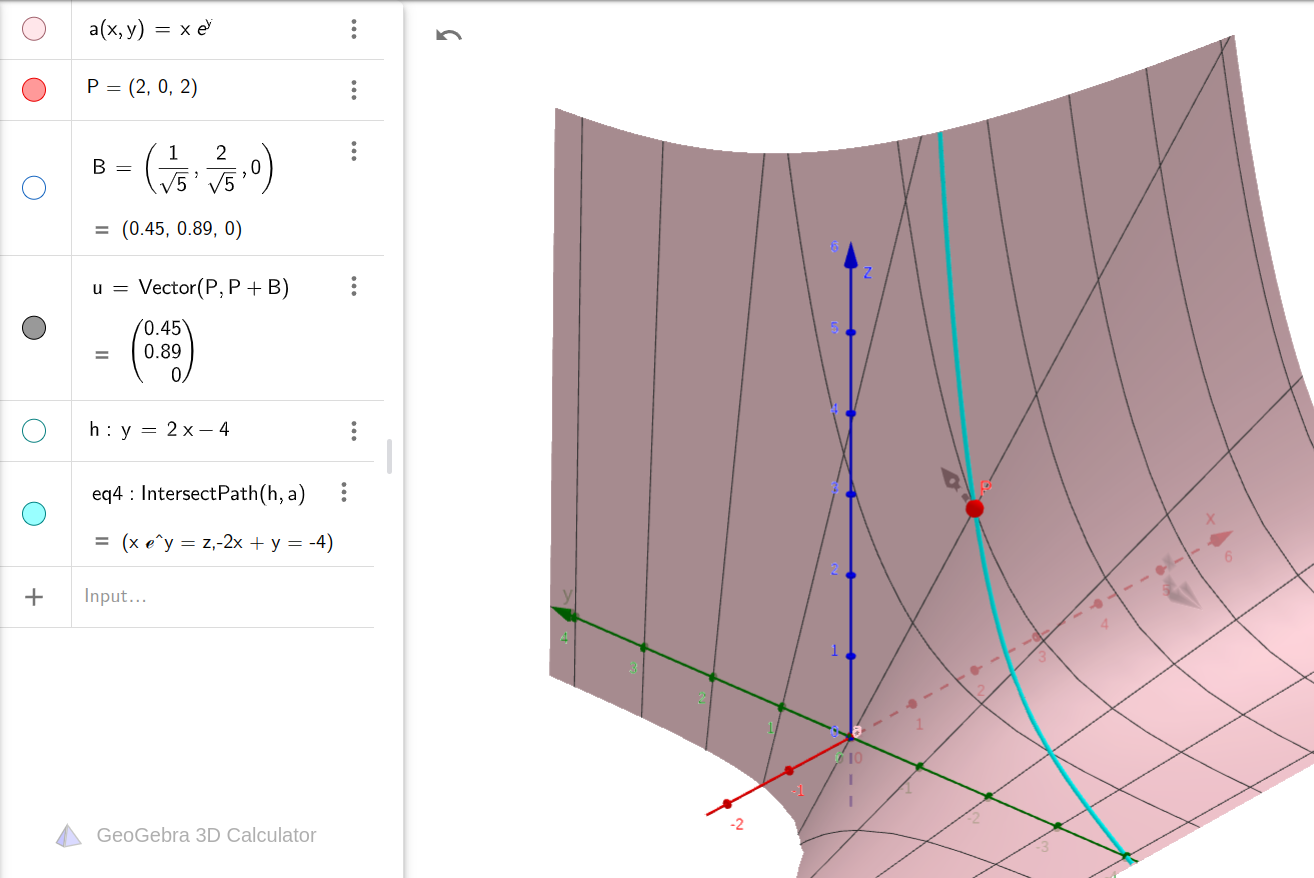
\includegraphics[width=0.95\textwidth]{gradiente-massima-pendenza.png}
\end{center}

\filbreak{}
\subsubsection*{Esercizio}

Derivare la seguente funzione composta \( f(\gamma(t))\) con:

\[
    f(x,y)= xe^{y}
\]
\[
    \gamma(t) = (x(t), y(t)) = (\cos (t) , \sin (t))
\]

\[
    F(t) = (f \circ \gamma) (t) = f(\gamma(t)) = \cos (t) e ^{\sin (t)}
\]

le derivate parziali sono:

\[
    \nabla f(x,y) = \left( \frac{\partial f}{\partial x}, \frac{\partial f}{\partial y} \right) = (e^{y}, xe^{y})
\]

\[
    \nabla f(\gamma(t)) = (e ^{\sin (t)}, \cos (t) e ^{\sin (t)})
\]

da cui:

\[
    F'(t) = \langle \nabla f(\gamma(t)), \gamma'(t) \rangle
\]

\[
    \gamma'(t) = (-\sin (t), \cos (t))
\]

quindi:

\[
    F'(t) = \left[ e ^{\sin(t)} (- \sin (t)) \right] + \left[ \cos (t) e ^{\sin (t)}\cos (t) \right] = e^{\sin(t)} \left( \cos^{2}(t) -\sin(t) \right)
\]

\pagebreak
\subsubsection{Derivate successive alla prima}

Sia \(f: A \subseteq \Rn \rightarrow \R \), con \(A\) aperto e \(f\) derivabile su \(A\)

Siano inoltre ben definite le derivate \(\frac{\partial f}{\partial x_i}(x,y) ~\forall i=1,\ldots,n\)

Definiamo cosa significa derivare ulteriormente questa funzione \(f\):

\defn{Derivate seconde}{ Se \(\exists \) sono della forma:

    \[
        \frac{\partial}{\partial x_j} \left( \frac{\partial f}{\partial x_i}(\ux) \right)(\ux)= \frac{\partial^{2} f}{\partial x_i \partial x_j}(\ux) = f_{x_i x_j}(\ux)
    \]

    e si ottengono al variare di \(i,j\) da \(1\) a \(n\).
}

\defn{Matrice Hessiana}{Attraverso le derivate seconde si ottiene una matrice \(n\times n\) che ha come elementi tutte le derivate seconde. Questa è chiamata matrice Hessiana e si indica con:

    \[
        Hf= \begin{bmatrix}
            \frac{\partial^{2} f}{\partial x_1 \partial x_1} & \frac{\partial^{2} f}{\partial x_1 \partial x_2} & \cdots & \frac{\partial^{2} f}{\partial x_1 \partial x_n} \\
            \frac{\partial^{2} f}{\partial x_2 \partial x_1} & \cdots                                           & \cdots & \cdots                                           \\
            \cdots                                           & \cdots                                           & \cdots & \cdots                                           \\
            \frac{\partial^{2} f}{\partial x_n \partial x_1} & \cdots                                           & \cdots & \frac{\partial^{2} f}{\partial x_n \partial x_n}
        \end{bmatrix} = \begin{bmatrix}
            f_{x_1 x_1} & f_{x_1 x_2} & \cdots & f_{x_1 x_n} \\
            f_{x_2 x_1} & \cdots      & \cdots & \cdots      \\
            \cdots      & \cdots      & \cdots & \cdots      \\
            f_{x_n x_1} & \cdots      & \cdots & f_{x_n x_n}
        \end{bmatrix}
    \]

}

\textbf{Nota:} se esistono tutte le derivate seconde di \(f\) nel punto \(\ux_0\), ovvero se è ben definita la matrice Hessiana, allora, si dice che \(f\) è \textbf{derivabile due volte in \(\ux_0\)}. Se questo vale per ogni punto \(\ux \) di un aperto \(A\), allora, si dice che f è \textbf{derivabile due volte in \(A\)}.

\defn{Derivate Pure}{
    Sono quelle che derivano per la stessa variabile, ovvero quelle che stanno sulla diagonale della matrice Hessiana:

    \[
        \frac{\partial^{2} f}{\partial x_i \partial x_i} = \frac{\partial^{2} f}{{(\partial x_i)}^{2}}
    \]

}

\defn{Derivate Miste}{
    Sono quelle che derivano per variabili diverse:

    \[
        \frac{\partial^{2} f}{\partial x_i \partial x_j}
    \]
}

\subsubsection*{Esempio matrice Hessiana per n=2}

\[
    Hf(x,y) = \begin{bmatrix}
        \displaystyle\frac{\partial^{2} f}{\partial x^{2}}(x,y)        & \displaystyle\frac{\partial^{2} f}{\partial x \partial y}(x,y) \\[5mm]
        \displaystyle\frac{\partial^{2} f}{\partial y \partial x}(x,y) & \displaystyle\frac{\partial^{2} f}{\partial y^{2}}(x,y)
    \end{bmatrix}
\]

\subsubsection*{Esercizio Matrice Hessiana}

Scrivere la matrice Hessiana di \(f(x,y)= xe ^{y}\):

Partiamo derivando per x:

\[
    f_x(x,y) = e ^{y}
\]

dunque:

\[
    f_{xx}(x,y) = 0
\]
\[
    f_{xy}(x,y) = e^{y}
\]

Partendo poi derivando per y:

\[
    f_y(x,y) = x e^{y}
\]

dunque:

\[
    f_{yx}(x,y) = e^{y}
\]
\[
    f_{yy}(x,y) = x e^{y}
\]

La matrice Hessiana di \(f(x,y)\) è dunque:

\[
    Hf = \begin{bmatrix}
        0      & e ^{y}  \\
        e ^{y} & x e^{y}
    \end{bmatrix}
\]

\pagebreak
\subsubsection{Teorema di Schwarz}

\teorema{Schwarz}{
    Sia \(f: A \subseteq \Rn \rightarrow \R \), \(A\) aperto;

    Sia, inoltre, \(f\) derivabile due volte su \(A\);

    Con \(\ux_0 \in A\), se le \(f_{x_i x_j}\) e le \(f_{x_j x_i}\) con \(i \neq j\) sono \textbf{continue} in \(\ux_0\), allora vale l'uguaglianza:

    \[
        f_{x_i x_j}(\ux_0) = f_{x_j x_i}(\ux_0)
    \]
}

Nota: Il teorema richiede solo che \(f\) sia continua in \(\ux_0\) non richiede che sia continua su tutto \(A\).

\;

Supponiamo però di essere nel caso di n=2 dove abbiamo anche che \(f\) è continua su tutto \(A\):
\[
    f \in C^{2} (A) \xrightarrow[]{\text{Schwarz}} f_{xy}(x,y) = f_{yx}(x,y) \quad \forall (x,y) \in A
\]

Inoltre, \(H f(x,y)\) è simmetrica \(\forall (x,y) \in A\), ovvero:
\[
    {(Hf(x,y))}^{T}=Hf(x,y)
\]

Più in generale, se abbiamo \(f \in C^{k}(A)\) allora l'ordine di derivazione non conta per le derivate parziali fino all'ordine \(k\).

Vediamo più nel dettaglio cosa succede nel caso di funzioni a due variabili.

\filbreak{}
\subsubsection*{Caso n=2}

Sia \(f: A \subseteq \R^{2} \rightarrow \R \), \(P_0=(x_0,y_0) \in A\), \(A\) aperto;

Sia \(f\) derivabile due volte su \(A\) (quindi esiste la matrice Hessiana);

Se le \(f_{xy}\) e \(f_{yx}\) sono continue in \((x_0,y_0)\), allora \(f_{xy}(x_0,y_0) = f_{yx}(x_0,y_0)\).

\begin{proof}
    Sia \(P_0=(x_0,y_0)\) e \(P=(x,y)\) un punto qualsiasi su \(A\), con \(P \neq P_0\)

    \begin{center}
        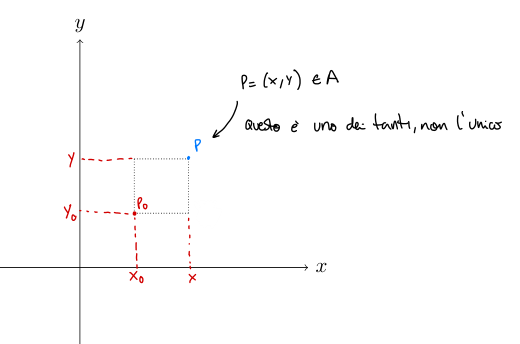
\includegraphics[width=0.55\textwidth]{teorema-di-schwarz-1.png}
    \end{center}

    Consideriamo il valore della funzione nei punti:
    \[
        f(x_0,y_0), f(x,y_0), f(x,y), f(x_0,y)
    \]

    e definiamo le seguenti funzioni che fissano una delle due variabili:
    \[
        F(x) = f(x,y) - f(x,y_0)
    \]
    \[
        G(y)  = f(x,y) - f(x_0,y)
    \]

    Con queste funzioni è evidente la seguente relazione:
    \[
        F(x) - F(x_0) = [f(x,y) - f(x,y_0)] - [f(x_0,y) -f(x_0,y_0)] = f(x,y) - f(x,y_0) - f(x_0,y) + f(x_0,y_0)
    \]
    \[
        G(y) - G(y_0) = [f(x,y) - f(x_0,y)] - [f(x,y_0) -f(x_0,y_0)] = f(x,y) - f(x_0,y) - f(x,y_0) + f(x_0,y_0)
    \]
    Quindi abbiamo che:
    \[
        F(x) - F(x_0) = G(y) -G(y_0)
    \]
    \filbreak{}
    Proviamo quindi a sviluppare le due parti singolarmente:
    \begin{itemize}
        \item Applico il teorema di Lagrange a \(F(x)\) nell'intervallo di estremi \((x_0, x)\), quindi si ha che esiste un punto \(x_1\) in questo intervallo per cui:

              \[
                  F(x)- F(x_0) = F'(x_1) (x-x_0)
              \]
              e dato che, \(F(x_1)=f(x_1,y)-f(x_1,y_0)\), posso arrivare a dire che:
              \[
                  F'(x_1) (x-x_0) = [f_x(x_1,y) - f_x(x_1,y_0) ] (x -x_0)
              \]

              Sappiamo che \(f\) è derivabile due volte, posso quindi applicare nuovamente Lagrange a \(f_x(x_1,y)\) nell'intervallo di estremi \((y_0,y)\). Quindi \(\exists y_1\) nell'intervallo tale che:

              \[
                  f_x(x_1,y) - f_x(x_1,y_0) = \frac{\partial }{\partial y}(f_x(x_1,y_1))(y-y_0) = f_{xy}(x_1,y_1)(y-y_0)
              \]

              quindi abbiamo fatto vedere che:

              \[
                  F(x)- F(x_0) = [f_{xy}(x_1,y_1)] (x-x_0) (y-y_0)
              \]
        \item Analogamente per \(G(y)\) applico Lagrange, quindi \(\exists y_2\) nell'intervallo \((y,y_0)\) tale che:

              \[
                  G(y) -G(y_0) = G'(y_2) (y-y_0) = [f_y(x,y_2) - f_y(x_0,y_2)] (y-y_0)
              \]

              applico nuovamente Lagrange a \(f_y(x,y_2)\) nell'intervallo \((x,x_0)\). Quindi \(\exists x_2 \in (x,x_0)\) t.c.:
              \[
                  f_y(x,y_2) - f_y(x_0,y_2) = f_{yx}(x_2,y_2)(x-x_0)
              \]
              infine quindi:
              \[
                  G(y) -G(y_0) = f_{yx}(x_2,y_2)(x-x_0)(y-y_0)
              \]
    \end{itemize}
    Ora, essendo \(F(x) - F(x_0) = G(y) - G(y_0)\), segue che:
    \[
        f_{xy}(x_1,y_1)(x-x_0)(y-y_0) = f_{yx}(x_2,y_2)(x-x_0)(y-y_0)
    \]

    e dato che per l'ipotesi iniziale \(P \neq P_0\), segue che \((x,y) \neq (x_0,y_0)\). Possiamo quindi semplificare le quantità non nulle, ovvero:
    \[
        f_{xy}(x_1,y_1) = f_{yx}(x_2,y_2)
    \]

    dove \((x_1,y_1)\) e \((x_2,y_2)\) stanno nell'intervallo del rettangolo tratteggiato del grafico iniziale.

    \filbreak{}
    Passando al limite per \(P \rightarrow P_0\), succede che:
    \[
        (x,y) \rightarrow (x_0,y_0)
    \]
    \[
        (x_1,y_1) \rightarrow (x_0,y_0)
    \]
    \[
        (x_2,y_2) \rightarrow (x_0,y_0)
    \]

    inoltre, ricordo che per il teorema di Lagrange:
    \[y_0 < y_1, y_2 < y\]
    \[x_0 < x_1, x_2 < x\]

    essendo, per ipotesi iniziale, le funzioni \(f_{xy},f_{yx}\) continue in \(P_0=(x_0,y_0)\), passando al limite di \(P \rightarrow P_0\) si ha dunque:
    \[
        f_{xy}(x_0,y_0) = f_{yx}(x_0,y_0)
    \]
\end{proof}

\pagebreak
\begin{proof} \textbf{Alternativa con integrali doppi}

    Sia un generico rettangolo \(R = [a,b]\times [c,d]\)

    Integro \(f_{xy}(x,y)\):

    \begin{spreadlines}{2mm}
        \begin{align*}
            \int_c^d \int_a^b {f_{yx}(x,y)} \diff{x}\diff{y} & = \int_c^d \int_a^b {(f_y(x,y))}_x \diff{x}\diff{y}               \\
                                                             & = \int_c^d \left[ f_y(b,y) - f_y(a,y) \right] \diff{y}            \\
                                                             & = \left[ f(b,d) - f(b,c) \right] + \left[ f(a,d) - f(a,c) \right]
        \end{align*}
    \end{spreadlines}

    Adesso vediamo l'altro integrale di \(f_{yx}(x,y)\) (si inverte l'integrale con il teorema di Fubini che presuppone che la funzione sia continua):

    \[
        \int_c^d \int_a^b f_{xy} \diff{x}\diff{y} \overset{\text{Teorema di Fubini}}{=} \int_a^b \int_c^d {(f_x)}_y \diff{y}\diff{x} =
    \]

    \[
        =\int_a^b \left[ f_x(x,d) - f_x(x,c) \right] \diff{x}  = [f(b,d) - f(a,d)] + [f(b,c) - f(a,c)]
    \]

    e quindi \(f_{xy}(x,y) = f_{yx}(x,y)\):

    \[
        f(b,d) - f(b,c) - f(a,d) + f(a,c) = f(b,d) - f(a,d) - f(b,c) + f(a,c)
    \]

    Questo funziona per ogni rettangolo che pongo infatti:

    \[
        \int_c^d \int_a^b f_{yx} \diff{x}\diff{y} = \int_c^d \int_a^b f_{xy} \diff{x}\diff{y}
    \]

    Quindi la loro differenza deve essere 0:

    \[
        \iint_R \underbrace{{(f_{yx} - f_{xy})}}_\text{continue} \diff{x}\diff{y} = 0
    \]

    Vale perché essendo le funzioni continue, se supponiamo per assurdo che la differenza sia positiva in un certo punto \(\ux_0\) allora la funzione è positiva anche in un piccolo rettangolo intorno a quel punto (per la continuità) ma questo è assurdo perché nel rettangolo la differenza delle due funzioni è 0.

    Quindi, il teorema di Schwarz funziona proprio per il fatto che le funzioni sono continue.

\end{proof}

\pagebreak
\subsubsection*{Esempio su Schwarz}

Usando il teorema di Schwarz, dire se la seguente funzione, \(f: \R^{2} \rightarrow \R \), è derivabile più di una volta, e in che punti:

\[
    f(x,y)=\begin{cases}
        0                                               & \text{se \((x,y) = (0,0)\)}    \\
        \displaystyle \frac{yx^{3}-xy^{3}}{x^{2}+y^{2}} & \text{se \((x,y) \neq (0,0)\)}
    \end{cases}
\]

Vediamo lo svolgimento per punti:
\begin{itemize}
    \item Prima cosa, verifichiamo che \(f(x,y)\) sia continua in \((0,0)\), ovvero che:

          \[
              \lim_{ (x,y) \to (0,0) } f(x,y)=f(0,0) = 0
          \]

          Passiamo in coordinate polari:
          \begin{align*}
              \frac{\rho\sin(\theta)\rho^3\cos^3(\theta) - \rho\cos(\theta)\rho^3\sin^3(\theta)}{\rho^2\cos^2\theta + \rho^2\sin^2\theta} & = \frac{\rho^4\left[ \sin(\theta)\cos^3(\theta) - \cos(\theta)\sin^3(\theta) \right]}{\rho^2}                \\
                                                                                                                                          & = \rho^2\sin(\theta)\cos(\theta) \left[ \cos^2(\theta) - \sin^2(\theta) \right] \xrightarrow[\rho \to 0]{} 0 \\
          \end{align*}
          Verifichiamo con il teorema del confronto:
          \begin{align*}
              \Big| \rho^2\sin(\theta)\cos(\theta) \left[ \cos^2(\theta) - \sin^2(\theta) \right] \Big| & \le \Big| \rho^2\sin(\theta)\cos(\theta) \left[ \cos^2(\theta) + \sin^2(\theta) \right] \Big| \\
                                                                                                        & \le \rho^2 \Big| \sin(\theta)\cos(\theta) \Big|                                               \\
                                                                                                        & \le \rho^2
          \end{align*}
          e dato che \(\rho^2 \xrightarrow[\rho \to 0]{} 0\), abbiamo verificato che \(f(x,y) \xrightarrow[(x,y) \to (0,0)]{} 0\), ovvero che \(f\) è continua in \((0,0)\).

    \item Ora, verifichiamo che anche le derivate parziali \(f_x(x,y)\) e \(f_y(x,y)\) siano continue in \((0,0)\):
          \begin{align*}
               & f_x(0,0) = \lim_{ h \to 0 } \frac{f(0+h,0) - f(0,0)}{h} = \lim_{ h \to 0 } \left( \frac{h^{3}\cdot0 - h\cdot 0}{h^{2}+0} - 0 \right) \cdot \frac{1}{h} = \lim_{ h \to 0 } \frac{0}{h} = 0 \\[2mm]
               & f_y(0,0) = \lim_{ h \to 0 } \frac{f(0,0+h) - f(0,0)}{h} = \cdots = 0
          \end{align*}

          \filbreak{}
    \item Calcoliamo le derivate parziali per \((x,y) \neq (0,0)\):
          \begin{align*}
               & f_x(x,y) = \frac{(3x^{2}y-y^{3})(x^{2}+y^{2})-(x^{3}y-xy^{3})(2x)}{{(x^{2}+y^{2})}^{2}} = \frac{x^{4}y+4x^{2}y^{3}-y^{5}}{{(x^{2}+y^{2})}^{2}} \\[2mm]
               & f_y(x,y) = \cdots = \frac{-xy^{4}-4x^{3}y^{2}+x^{5}}{{(x^{2}+y^{2})}^{2}}
          \end{align*}

    \item ricordando da sopra che \(f_x(0,0)=0=f_y(0,0)\), calcoliamo le derivate seconde in \((0,0)\):
          \[
              f_{xy} (0,0) = \lim_{ k \to 0 } \frac{f_x(0,0+k) - f_x(0,0)}{k} = \lim_{ k \to 0 } \frac{ \left( \frac{-k^{5}}{k^{4}} \right) - (0)}{k} = \lim_{ k \to 0 } - \frac{k}{k} = -1
          \]
          \[
              f_{yx}(0,0) = \lim_{ k \to 0 } \frac{f_y(0+k,0) - f_y(0,0)}{k} = \lim_{ k \to 0 } \frac{ \left( \frac{k^{5}}{k^{4}} \right) - (0)}{k} = \lim_{ k \to 0 } \frac{k}{k} = 1
          \]
\end{itemize}

Possiamo quindi dire che la funzione \(f(x,y)\) è derivabile due volte su \((0,0)\), ma che \(f(x,y) \notin C^2(A)\). Questo perché le derivate seconde sono diverse e quindi per il teorema di Schwarz le derivate seconde non sono continue in \((0,0)\).

\newpage
\subsection{Approssimazioni lineari}

\subsubsection{Introduzione all'approssimazione tramite Taylor}

Sia \(A \subseteq \Rn \) con \(A\) aperto;

Sia \(f: A \subseteq \Rn \rightarrow \R \), di classe \(C^{k}\) per qualche \(k \in \N \);

Siano \(\ux \) e \(\ux +\uh \) due punti in \(A\) tali che il segmento \([\ux, \ux +\uh ] \subset \Rn \) sia tutto contenuto in \(A\).

Definiamo la funzione \(x(t) : \R \to \Rn \), che associa \(t \mapsto \ux+t\uh \) definita \(\forall t \in [0,1]\).

Possiamo quindi scrivere gli elementi del segmento come:
\[
    [\ux , \ux +\uh ] = \{x(t) ~\forall t \in [0,1]\} \subset \Rn
\]

Definiamo inoltre la funzione \(F(t) : [0,1] \to \R \), che associa \(t \mapsto f(x(t)) = f(\ux+t\uh)\)

Se \(f \in C^{1}\), allora anche \(F \in C^1\), quindi esiste:

\[
    F'(t) = [f(x(t))]' = \prods{\nabla f(x(t))}{\frac{\diff }{\diff t}x(t)} = \prods{\nabla f(\ux+t\uh)}{\uh} = \sum^{n}_{i=1} \left[ \frac{\partial f}{\partial x_i} (\ux + t\uh ) \right] h_i
\]

Se inoltre, \(f \in C^{2}\), allora esiste anche:

\[
    F''(t) = \left( F'(t) \right)' = \sum^{n}_{j=1} \frac{\partial}{\partial x_j} \left[ \sum^{n}_{i=1} \frac{\partial f}{\partial x_i}(\ux + t\uh ) h_i \right] h_j = \sum^{n}_{i,j=1} \left[ \frac{\partial^{2} f}{\partial x_i \partial x_j} (\ux +  t\uh ) \right] h_i h_j
\]

Questo è un polinomio quadratico.

\pagebreak
\subsubsection{Polinomio di Taylor con resto di Lagrange}

Ridefiniamo quanto detto nell'introduzione:
\begin{itemize}
    \item Sia \(A \subseteq \Rn \) con \(A\) aperto;

    \item Sia \(f: A \subseteq \Rn \rightarrow \R \), di classe \(C^{k}\) per qualche \(k \in \N \);

    \item Siano \(\ux \) e \(\ux +\uh \) due punti in \(A\) tali che il segmento \([\ux, \ux +\uh ] \subset \Rn \) sia tutto contenuto in \(A\).

    \item Definiamo la funzione \(x(t) : \R \to \Rn \), che associa \(t \mapsto \ux+t\uh \) definita \(\forall t \in [0,1]\). Con questa, il segmento è possibile scriverlo come:
          \[
              [\ux , \ux +\uh ] = \{x(t) ~\forall t \in [0,1]\} \subset \Rn
          \]

    \item Definiamo inoltre la funzione \(F(t) : [0,1] \to \R \), che associa \(t \mapsto f(x(t)) = f(\ux+t\uh)\)
\end{itemize}

Osserviamo che \(F(0) = f(\ux)\) e che \(F(1) = f(\ux+\uh)\).

\proposizione{Formula di Taylor con resto di Lagrange}{
    Essendo \(F\) una funzione in una variabile, applico Taylor in una variabile fino all'ordine \((k-1)\), usando il resto di Lagrange (rappresentato dentro il box).

    Quindi, centrando il polinomio di Taylor in \(0\), esiste \(\theta \in (0,1)\) tale che vale:
    \begin{align*}
        F(1) & = F(0) + F'(0)(1-0) + \frac{F''(0)}{2}{(1-0)}^{2} + \cdots + \frac{F^{(k-1)}(0)}{(k-1)!}{(1-0)}^{k-1} + \boxed{\frac{F^{(k)}(\theta)}{k!}{(1-0)}^{k}} \\
             & = F(0) + F'(0) + \frac{F''(0)}{2} + \cdots + \frac{F^{(k-1)}(0)}{(k-1)!} + \boxed{\frac{F^{k}(\theta)}{k!}}
    \end{align*}
}

Vediamo dunque di dimostrare quanto appena detto per i primi ordini:

\filbreak{}
\subsubsection*{Per k=1}

Con \(k=1\) ritroviamo una versione in più variabili del teorema di Lagrange.

\teorema{Formula di Taylor di ordine 1 con resto in forma di Lagrange}{
    Date tutte le definizione iniziali;
    Se \(f \in C^1\), allora esiste \(\theta \in (0,1)\) tale che:
    \begin{align*}
        f(\ux+\uh) & = f(\ux) + f_x(\theta)\cdot\uh                                                                    &                         \\
                   & = f(\ux) + \underbrace{\prods{\nabla f(\ux+ \theta \uh)}{\uh}}_{\text{resto calcolato nel punto}} & \text{(forma compatta)} \\
                   & = f(\ux) + \sum^{n}_{i=1} \frac{\partial f}{\partial x_i}(\ux+\theta\uh) \cdot h_i                & \text{(forma estesa)}
    \end{align*}
}
\begin{proof}
    Applichiamo Lagrange a \(F\) nell'intervallo \((0,1)\); \(\exists \theta \in (0,1)\) tale che:

    \[
        F'(\theta) = \frac{F(1) - F(0)}{1-0} \implies F(1) = F(0) + F'(\theta)
    \]

    Ricordando che \(F'(t) = \prods{\nabla f(\ux+t\uh)}{\uh}\), e che \(F(0) = f(\ux)\), e che \(F(1) = f(\ux+\uh)\); sostituendo, ritroviamo la tesi:

    \[
        f(\ux+\uh) = f(\ux) + \prods{\nabla f(\ux+ \theta \uh)}{\uh}
    \]

\end{proof}

\subsubsection*{Per k=2}

\teorema{Formula di Taylor di ordine 1 con resto in forma di Lagrange}{
    Date tutte le definizione iniziali;
    Se \(f \in C^2\), allora esiste \(\theta \in (0,1)\) tale che:
    \begin{align*}
        f(\ux+\uh) & = f(\ux) + \sum^{n}_{i=1} \left[ \frac{\partial f}{\partial x_i}(\ux) \cdot h_i \right] + \frac{1}{2}\sum^{n}_{i,j=1} \left[ \frac{\partial^{2} f}{\partial x_i \partial x_j}(\ux+\theta\uh) \cdot h_i h_j \right] \\
                   & = f(\ux) + \prods{\nabla f(\ux)}{\uh} + \frac{1}{2}\prods{Hf(\ux+\theta\uh) \cdot \uh}{\uh}
    \end{align*}
}
\begin{proof}
    Come per il caso precedente, la tesi viene da Taylor per \(k=2\):

    \[
        F(1) = F(0) + F'(0) + \frac{F''(\theta)}{2}
    \]

\end{proof}

\pagebreak
\subsubsection{Polinomio di Taylor con resto di Peano}

\defn{Resto di Peano in \(\Rn \)}{
    Date tutte le definizione iniziali;
    Se \(f \in C^2\), allora:

    \[
        f(\ux+\uh) = f(\ux) + \langle \nabla f(\ux),\uh \rangle + \frac{1}{2} \langle Hf(\ux) \cdot \uh, \uh \rangle + o(\norm{\uh}^2)
    \]
}

\defn{Resto di Peano in \(\R^2\)}{
    Date tutte le definizione iniziali;

    Siano \(\ux_0 =(x_0,y_0)\), \(\uh  = (h,k)\);

    Sia \(f \in C^2(A)\) tale che esista \(Hf(x,y) ~\forall (x,y) \in A\), dove quindi \(Hf(x,y)\) è simmetrica.

    Se tutto questo, allora:
    \begin{align*}
        f(x_0 + h, y_0 + k) = & \ f(x_0,y_0)                                                                                                       \\
                              & + f_x(x_0,y_0) \cdot h + f_y(x_0,y_0) \cdot k                                                                      \\
                              & + \frac{1}{2} \left[ f_{xx}(x_0,y_0) \cdot h^{2} + 2f_{xy}(x_0,y_0) \cdot hk + f_{yy}(x_0,y_0) \cdot k^{2} \right] \\
                              & + o(h^{2}+k^{2})
    \end{align*}
}
Il pezzo tra parentesi quadre è il risultato del prodotto tra matrici e vettori:
\begin{align*}
    \begin{bmatrix}
        f_{xx} & f_{xy} \\
        f_{xy} & f_{yy}
    \end{bmatrix}
    \cdot
    \begin{bmatrix}
        h \\
        k
    \end{bmatrix}
    \cdot
    \begin{bmatrix}
        h & k
    \end{bmatrix}
     & =
    \begin{bmatrix}
        f_{xx} \cdot h + f_{xy} \cdot k \\
        f_{xy} \cdot h + f_{yy} \cdot k
    \end{bmatrix}
    \cdot
    \begin{bmatrix}
        h & k
    \end{bmatrix}                                                                       \\
     & = (f_{xx} \cdot h + f_{xy} \cdot k)(h+k) + (f_{xy} \cdot h + f_{yy} \cdot k)(h+k) \\
\end{align*}
Quindi, \(\boxed{P_2(\ux, \ux_0)}\) è il polinomio omogeneo in due variabili, di grado 2, che meglio approssima la funzione \(f\) vicino a \(\ux_0\). Ovvero, per la definizione di o piccolo:
\[
    \lim_{\ux \to \ux_0} \frac{f(x,y) - P_2(x,y)}{\underbrace{{(x-x_0)}^2 + {(y-y_0)}^2}_{\norm{\ux-\ux_0}^2}} = 0
\]
In \(\ux_0 = (x_0,y_0)\) possiamo quindi approssimare la funzione come:

\[
    f(x,y) = P_2((x,y), (x_0, y_0)) + o({(x-x_0)}^{2} + {(y-y_0)}^{2})
\]
con:
\begin{align*}
    P_2(\ux, \ux_0) = & \ f(x_0,y_0) + f_x(x_0,y_0) (x-x_0) + f_y(x_0,y_0) (y-y_0)                                                                      \\
                      & + \frac{1}{2} \left[ [f_{xx}(x_0,y_0)]{(x-x_0)}^{2} + 2[f_{xy}(x_0,y_0)](x-x_0)(y-y_0) + [f_{yy}(x_0,y_0)]{(y-y_0)}^{2} \right]
\end{align*}

\newpage
\subsection{Massimi e minimi}

\subsubsection{Massimi e minimi locali}

Vediamo ora alcuni concetti che ci serviranno poi per i problemi di ottimizzazione vincolata.

\defn{Massimo e minimo locale}{

    Sia \(f: D \subseteq \Rn \to \R \), dove \(D\) è il dominio, ovvero l'unione dei punti dell'insieme aperto con quelli della frontiera.

    Si dice che \(\ux_0 \in D\) è un punto di \textbf{minimo locale} (o \textbf{relativo}), se esiste un intorno sferico \(B(\ux_0, \sigma) \), con \(\sigma > 0\), tale che:

    \[
        f(\ux_0) \le f(\ux) \quad \forall \ux \in D \cap B(\ux_0, \sigma)
    \]

    La definizione è analoga per il punto di massimo locale.
}

\defn{Massimo/Minimo stretto}{
    Il punto di minimo o massimo locale si dice \textbf{stretto} se la disuguaglianza è strettamente minore o strettamente maggiore.
}

\defn{Massimo/Minimo globale}{
    Un punto di massimo/minimo, si dice \textbf{globale} (o \textbf{assoluto}) se la disuguaglianza vale per tutto il dominio, ovvero \(\forall \ux \in D\) e non solo per l'intorno sferico di centro \(\ux_0\) e di raggio \(\sigma \).
}

Da Analisi 1 sappiamo che i punti di minimo e massimo vanno ricercati fra i punti stazionari, ovvero nei punti critici, di funzioni differenziabili, in cui il gradiente si annulla.

Se \(\ux_0\) è punto di minimo (massimo) locale interno a \(D\) (quindi \(\ux_0 \in D\)) allora vale l'estensione in più variabili del Teorema di Fermat.

\filbreak{}
\teorema{Teorema di Fermat per funzioni in più variabili}{
    Sia \(f:D \subset \Rn \to \R \);

    Sia \(\ux_0 \in D\) punto di estremo locale per \(f\);

    Se \(f\) è differenziabile in \(\ux_0\), allora, \(\nabla f(\ux_0) = 0\)
}
\begin{proof}
    Supponiamo \(\ux_0\) punto di massimo relativo. Allora \(\ux_0\) è punto di massimo relativo anche per la restrizione di \(f\) lungo una qualsiasi retta passante per \(\ux_0\).

    Consideriamo il versore \(\underline{v} \in \Rn \) come il vettore di norma 1 che ci indica la direzione di tale retta passante per \(\ux_0\). I punti su tale retta sono quindi della forma \(\ux_0 + t\underline{v}\) per \(t \in \R \).

    Definiamo la funzione \(F: \R \to \R \) che associa \(t \mapsto f(\ux_0 + t\underline{v})\). Questa funzione \(F(t)\), è una funzione in \textbf{una variabile} e diciamo che sia almeno definita in un intorno di \(t=0\).

    Ora, siccome \(\ux_0\) è punto di massimo per \(f\), allora in \(t=0\) abbiamo un punto di massimo per \(F\). Quindi per il teorema di Fermat in una variabile: \(F'(0) = 0\).

    Se quindi espandiamo \(F'(t)\) con la regola della catena, per qualsiasi direzione \(\underline{v}\) otteniamo:

    \[
        F'(t) = \prods{\nabla f(\ux + t\underline{v})}{\underline{v}}
    \]
    \[
        F'(0) = 0 = \prods{\nabla f(\ux_0)}{\underline{v}}
    \]

    E siccome \(\norm{\underline{v}} = 1\), allora \(\underline{v} \neq \uzero \), allora necessariamente \(\nabla f(\ux_0) = 0\).

\end{proof}

\filbreak{}
\defn{Punti stazionari (o critici)}{
    I punti \(\ux_0 \in A\) tali che \(\nabla f(\ux_0) = 0\) si dicono \textbf{punti stazionari} (o critici) di \(f\) in \(A\).
}

\defn{Sella (o colle)}{
    Essere un punto stazionario, è condizione necessaria ma non sufficiente per essere un punto di estremo.

    In funzioni a una variabile, un punto stazionario che non era però un punto di estremo lo chiamavamo flesso;

    In funzioni a più variabili, un punto stazionario che non è però un estremo relativo viene chiamato \textbf{sella} (o colle).
}

Un esempio classico di punto di sella, è il punto \((0,0,0)\) nella funzione \(z=x^2-y^2\):
\begin{center}
    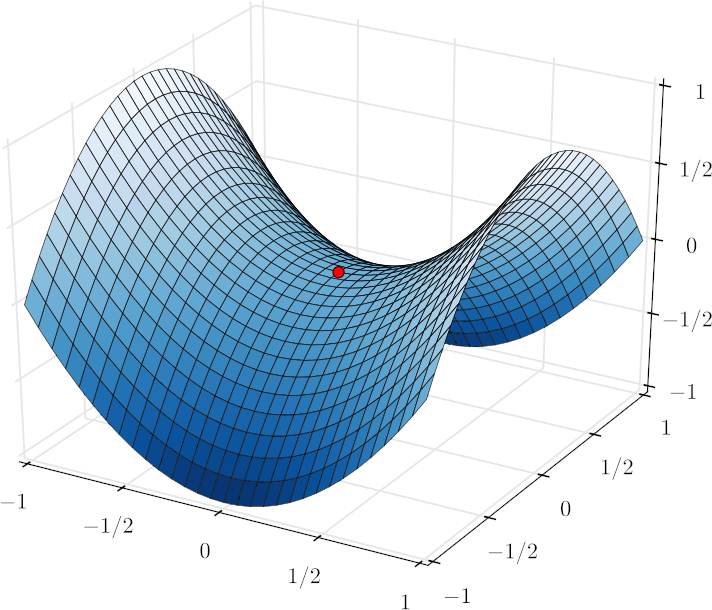
\includegraphics[width=0.5\textwidth]{punto-di-sella.png}
\end{center}

\filbreak{}
\subsubsection*{Esercizio 1}

Cercare i punti critici della seguente funzione:

\[
    f(x,y) = 2x^{2} - 2xy +y^{2}
\]

Cerco i punti dove \(\nabla f(x,y) = 0\):
\begin{align*}
     & f_x = 4x -2y  \\
     & f_y = -2x +2y
\end{align*}

\[
    \begin{cases}
        4x -2y = 0 \\
        -2x +2y = 0
    \end{cases}
    \implies
    \begin{cases}
        x = 0 \\
        y = 0
    \end{cases}
\]

Quindi, \(\ux_0 = (0,0)\), è un punto critico \(\implies \nabla f(\ux_0)=0\)

Inoltre, possiamo osservare che:

\[
    f(x,y) = x^{2} + {(x-y)}^{2}
\]

è una somma di due quadrati, quindi:

\[
    f(x,y) > f(0,0) ~\forall (x,y) \neq (0,0)
\]

Quindi si ha che \(\ux_0 = (0,0)\) è un punto di \textbf{minimo globale stretto}.

\subsubsection*{Esercizio 2}

Cercare i punti critici della seguente funzione:

\[
    f(x,y) = x^{2}-y^{2}
\]

\[
    \nabla f(x,y) = (2x, -2y)
\]

anche qui \((0,0)\) è l'unico punto critico. Questo punto è però un punto di sella, infatti, se consideriamo gli incrementi lungo gli assi:
\begin{itemize}
    \item Lungo l'asse x: \(f(x,0) = x^{2} \ge 0 ~\forall x\)
    \item Lungo l'asse y: \(f(0,y) = -y^{2} \le 0 ~\forall y\)
\end{itemize}
abbiamo un cambiamento di segno dentro l'intorno sferico \(B(\uzero, r)\) e quindi \(\ux_0\) non è ne un massimo ne un minimo.

Come vedremo tra poco, questa conclusione è possibile trarla anche facendo un'analisi dell'incremento subito dalla funzione:
\[
    \Delta f(x,y) = f(x,y) - f(0,0) = x^{2}-y^{2}-0 \quad\forall (x,y) \in B(\uzero,r),\ r>0
\]
da cui si nota che a seconda del valore di \((x,y)\) si ha un cambiamento di segno, e quindi abbiamo un punto di sella.

\pagebreak
\subsubsection{Forma quadratica}

Prima di passare al prossimo argomento è necessario introdurre la notazione di ``Forma quadratica''.

Per un vettore \(\ux \in \Rn \), una forma quadratica è un polinomio omogeneo di secondo grado nelle variabili \((x_1,\ldots,x_n)\):

\[
    q(\ux ) = q(x_1,\ldots,x_n) = \sum^{n}_{i,j=1} a_{ij} x_i x_j
\]

Quindi, se consideriamo la matrice dei coefficienti \(A = (a_{ij})\), possiamo scrivere ogni forma quadratica come:

\[
    q(\ux ) = \prods{A\ux}{\ux}
\]

Da qui, notiamo che tutti gli \({x_i}^{2}\) hanno come coefficiente \(a_{ii}\), ovvero i coefficienti che stanno sulla diagonale di \(A\).

\subsubsection*{Esempio}

Sia \(n=2\); \(\ux =(x_1,x_2)\); \(A\) simmetrica.

Sappiamo in generale che:

\[
    q(x_1,x_2) = a_{11} {x_1}^{2} + 2a_{12} x_1 x_2 + a_{22}{x_2}^{2}
\]

per una matrice \(2\times 2\):

\[
    A= \begin{pmatrix}
        1 & 5 \\
        5 & 4
    \end{pmatrix} \iff
    q(x_1,x_2) = {x_1}^{2}+4 {x_2}^{2}+ 10 x_1 x_2
\]

per una matrice \(3\times 3\):

\[
    A = \begin{pmatrix}
        2  & -2 & 5 \\
        -2 & 3  & 0 \\
        5  & 0  & 4
    \end{pmatrix} \iff
    q(\ux ) = 2 {x_1}^{2}+3 {x_2}^{2}+ 4 {x_3}^{2} - 4 x_1 x_2 + 10 x_1 x_3
\]

\subsubsection*{Definizione sul segno}

Sia \(n=2\); per una data matrice dei coefficienti \(A = (a_{ij})\); la forma quadratica \(q: \ux \mapsto \prods{A\ux}{\ux}\)
\begin{itemize}
    \item si dice \textbf{definita positiva} se \(\forall \ux \neq 0\) si ha \(q(\ux ) >0\)
    \item si dice \textbf{definita negativa} se \(\forall \ux \neq 0\) si ha \(q(\ux ) <0\)
    \item si dice \textbf{indefinita} se \(\exists x_1, x_2 \in \R^{2} \giventhat q(x_1) < 0 < q(x_2)\), ovvero cambia il segno
\end{itemize}

\pagebreak
\subsubsection{Classificazione dei punti critici {-} Matrice Hessiana}

\proposizione{Test dell'hessiana}{

Sia \(f: D \subseteq \R^{2} \to \R \), \(D\) aperto con \(f \in C^{2}(D)\)

Sia \((x_0,y_0) \in D\) un punto critico per \(f\), ovvero tale che \(\nabla f(x_0,y_0) = 0\)

Sia il determinante della matrice Hessiana \(\neq 0\), ovvero:
\[
    \det (Hf(x_0,y_0)) =
    \left| \begin{matrix}
        f_{xx}(x_0,y_0) & f_{xy}(x_0,y_0) \\
        f_{xy}(x_0,y_0) & f_{yy}(x_0,y_0)
    \end{matrix} \right| =
    f_{xx}(x_0,y_0) f_{yy}(x_0,y_0) - {f_{xy}}^{2}(x_0,y_0)
    \neq 0
\]

Allora:

\begin{itemize}
    \item Se \(\det(Hf(x_0,y_0))>0\) e \(f_{xx}(x_0,y_0)>0 \implies (x_0,y_0)\) è punto di minimo locale
    \item Se \(\det(Hf(x_0,y_0))>0\) e \(f_{xx}(x_0,y_0)<0 \implies (x_0,y_0)\) è punto di massimo locale
    \item Se \(\det(Hf(x_0,y_0))<0 \implies (x_0,y_0)\) è un punto di sella
\end{itemize}
}

Osservazione: se \(\det(Hf(x_0,y_0)) =0\) il test dell'hessiana \textbf{non} ci fornisce informazioni. Devo quindi fare un'analisi diretta dell'incremento subito dalla funzione, ovvero:
\[
    \Delta f(x,y) = f(x,y)-f(x_0,y_0) \qquad \forall (x,y) \in D \cap B(x_0,y_0)
\]

\begin{proof}
    Questa dimostrazione è basata sull'approssimazione al secondo ordine della nostra funzione in \(\ux = (x_0, y_0)\), attraverso la formula di Taylor al II ordine col resto di Peano:

    \[
        f(\ux + \uh ) = f(\ux ) + \prods{ \nabla f(\ux )}{\uh} + \frac{1}{2} \prods{ Hf(\ux ) \cdot \uh}{\uh} + o(\norm{\uh}^{2})
    \]

    Se consideriamo l'approssimazione nel punto \(\ux = (x_0,y_0)\), ricordando che per ipotesi \(\ux \) è punto critico e quindi \(f_x(\ux)=0=f_y(\ux)\), abbiamo dunque che:
    \begin{align*}
        f(\ux + \uh)          & = f(\ux) + 0 + \frac{1}{2} \prods{ Hf(\ux ) \cdot \uh}{\uh} + o({\norm{\uh}}^2) \\
        f(\ux + \uh) - f(\ux) & = \frac{1}{2} \prods{ Hf(\ux ) \cdot \uh}{\uh} + o({\norm{\uh}}^2)              \\[2mm]
        f(x,y) - f(x_0,y_0)   & = \frac{1}{2} \prods{ Hf(\ux ) \cdot \uh}{\uh} + o({\norm{\uh}}^2)
    \end{align*}
    Osserviamo che, \(\frac{1}{2} \prods{ Hf(\ux ) \cdot \uh}{\uh}\), è un polinomio di II grado in \(\uh=(h,k)\), i cui coefficienti sono le derivate seconde di \(f\), che esistono per ipotesi.

    In generale, questo polinomio è sempre una forma quadratica, \(q(\uh)\) con {\(\uh \in \Rn \)}, quindi un polinomio omogeneo di secondo grado nelle variabili \((h_1,\ldots,h_n)\).

    Ricordando che \(q(\uh) = \prods{A\uh}{\uh}\), nel nostro caso la matrice associata \(A\) è proprio la matrice Hessiana, che è pure simmetrica per il teorema di Schwarz (ipotesi iniziali: \(f \in C^{2}(D)\)).

    Studiare il segno di \(\Delta f(x,y)\), ovvero il segno della funzione nell'intorno del punto critico, è quindi uguale a studiare il segno di questa quadratica hessiana.

    Per la regola di Cartesio, per studiare il segno della quadratica hessiana possiamo usare il segno degli autovalori. Vediamo quindi cosa succede:

    \begin{itemize}
        \item \(\det(Hf(\ux))>0,\ f_{xx}(\ux)>0 \implies \) forma quadratica è definita positiva \(\implies \ux \) è minimo
        \item \(\det(Hf(\ux))>0,\ f_{xx}(\ux)<0 \implies \) forma quadratica è definita negativa \(\implies \ux \) è massimo
        \item \(\det(Hf(\ux))<0 \implies \) forma quadratica è indefinita \(\implies \ux \) è punto di sella
    \end{itemize}

\end{proof}

\subsubsection*{Esercizio 1}

Classificare i punti critici delle seguenti funzioni:

\[
    f(x,y) = 2x^{3}-6xy + 3y^{2}
\]

\[
    \nabla f(x,y)=0 \implies \begin{cases}
        6x^{2}-6y=0 \\
        -6x + 6y =0
    \end{cases}
    \implies
    (x,y) \in \{(0,0), (1,1)\}
\]

Test dell'hessiana:

\[
    f_{xx}(x,y) = 12x
\]
\[
    f_{xy}(x,y) = -6
\]
\[
    f_{yy}(x,y) = 6
\]

quindi:

\[
    H f(x,y) = \begin{bmatrix}
        12x & -6 \\
        -6  & 6
    \end{bmatrix}
\]

gli sostituiamo i punti trovati prima:

\[
    Hf(0,0) = \begin{bmatrix}
        0  & -6 \\
        -6 & 6
    \end{bmatrix}
\]

quindi:

\[
    \det (Hf(0,0)) = -36 <0 \implies (0,0) \text{ punto di sella}
\]

\[
    Hf(1,1) = \begin{bmatrix}
        12 & -6 \\
        -6 & 6
    \end{bmatrix}
\]

quindi:

\[
    \det (Hf(1,1)) = 36 >0 \text{ e } f_{xx}(1,1) = 12 > 0 \implies (0,0) \text{ minimo locale}
\]

\subsubsection*{Esercizio 2}

\[
    f(x,y) = x^{3} + {(x-y)}^{2}
\]

\[
    \nabla f(x,y)=0
    \implies
    \begin{cases}
        3x^{2}+2(x-y) = 0 \\
        -2(x-y) = 0
    \end{cases}
    \implies
    \begin{cases}
        3x^{2}= 0 \\
        x-y= 0
    \end{cases}
    \implies
    (x,y) \in \{(0,0)\}
\]

\[
    f_{xx}(x,y) = 6x+2
\]
\[
    f_{xy}(x,y) = -2
\]
\[
    f_{yy}(x,y) = 2
\]

\[
    H f(x,y) = \begin{bmatrix}
        6x+2 & -2 \\
        -2   & 2
    \end{bmatrix}
\]

\[
    \det(H f(x,y)) = 2(6x+2) - 4
\]
\[
    \det(H f(0,0)) = 4-4 = 0
\]

Quindi non posso applicare il test dell'hessiana.

Allora considero l'incremento in un intorno sferico dell'origine:

\[
    \Delta f(x,y) = f(x,y) - f(0,0) = x^{3}+{(x-y)}^{2} -0 = x^{3}+{(x-y)}^{2}
\]

e dunque, si può escludere che in \((0,0)\) ci sia minimo o massimo relativo perché il segno cambia.

Infatti, questo si vede facilmente ad esempio restringendo la funzione lungo la curva \(y=x\):

\[
    \Delta f(x,x) = x^{3}
\]

questa cambia segno dipendentemente dal valore di \(x\).

Quindi possiamo concludere che \((0,0)\) è un punto di sella.

\pagebreak
\subsubsection{Massimi e minimi su domini limitati e chiusi di \texorpdfstring{\(\R^{2}\)}{R2}}

Nel caso di funzioni su domini limitati e chiusi vale il seguente teorema:

\teorema{Weierstrass}{
    Sia \(f: K \subseteq \R^2 \to \R \) continua; con \(K\) \textbf{limitato e chiuso}.

    Allora \(f\) è \textbf{limitata} e ha minimo e massimo su \(K\), ovvero:

    \[
        \exists (x_0,y_0),(x_1,y_1) \in K \giventhat f(x_0,y_0) \le f(x,y) \le f(x_1, y_1) ~\forall (x,y) \in K
    \]

    ovvero, esiste:
    \begin{itemize}
        \item \(f(x_0, y_0)\) valore minimo assoluto di \(f\) su \(K\)
        \item \(f(x_1, y_1)\) valore massimo assoluto di \(f\) su \(K\)
    \end{itemize}
}

\newpage
\subsection{Ottimizzazione vincolata}

\subsubsection{I problemi di ottimizzazione}

I problemi di ottimizzazione consistono nella ricerca di punti stazionari (o critici) di una funzione ad n variabili.

Nel caso di ricerca di massimi, minimi o punti di sella in un intero insieme numerico, parliamo di \textbf{ottimizzazione libera} (o lineare). Ovvero, si procede cercando tutti i punti critici (massimi, minimi e selle) nel dominio della funzione.

Il sistema da analizzare può essere però soggetto a vincoli, per cui si parla di \textbf{ottimizzazione vincolata}. Con vincolo si intende una condizione matematica da rispettare che nel nostro caso prende la forma di equazioni e/o disequazioni matematiche. Dobbiamo quindi trovare i punti critici solamente all'interno dello spazio che rispetta questi vincoli.

In questi appunti noi ci occuperemo solo di problemi di ottimizzazione vincolata in 2 variabili con un 1 vincolo sotto forma di equazione.

Anche se nel nostro caso sembreranno ridondanti, vedremo due metodi per risolvere questo tipo di problema. L'importanza dell'esistenza di entrambi serve per quando non si lavora più con sole funzioni a due variabili e un solo vincolo, che però non vedremo in questi appunti.

Un'altra importante osservazione è che i seguenti metodi funzionano solo quando i vincoli sono nella forma di equazioni. In questo caso specifico dobbiamo trovare i punti critici lungo una curva delineata dall'intersezione della nostra funzione con quella del vincolo.

I due metodi che vedremo sono dunque:
\begin{itemize}
    \item \textbf{Metodo di parametrizzazione}:

          Attraverso la parametrizzazione della curva del vincolo ci ritroviamo a studiare una funzione in una singola variabile.

    \item \textbf{Metodo dei moltiplicatori di Lagrange}:

          Attraverso un'osservazione geometrica dei gradienti delle due funzioni, definiamo una relazione che implica la presenza di un punto critico.

          In questo metodo, a differenza del precedente, non è necessario parametrizzare alcuna curva. Qui, si lavora con i gradienti delle funzioni.
\end{itemize}

\pagebreak
\subsubsection{Metodo di parametrizzazione}

Sia \(f: A \subseteq \R^2 \to \R \) una funzione \(\in C^1(A)\);

Vogliamo cercare gli estremi della funzione \(f\) su una specifica curva
\[\gamma : I \subseteq \R \to A\]
definita da un'equazione del tipo:
\[
    g(x,y) = k
\]

Questa funzione \(g(x,y) \in C^{1}(A)\) definisce il nostro vincolo, e i punti della funzione \(f\) che rispettano il vincolo, ovvero quelli che sono sulla curva \(\gamma \) possiamo rappresentarli con l'insieme:

\[
    V = \left\{ (x,y) \in A \giventhat g(x,y) = k \right\}
\]

Se \(g\) è parametrizzabile come \(\gamma(t) = (\gamma_1(t), \gamma_2(t))\) con \(t \in I\), possiamo allora studiare la funzione composta:

\[
    h(t) = (f \circ \gamma) (t) = f(\gamma(t)) \quad \text{con } t \in I
\]

La funzione composta \(h\) è una funzione nella sola variabile \(t\) e rappresenta la funzione \(f\) ristretta alla curva \(\gamma \). Per determinare i punti estremali di \(f\) ristretta alla curva \(\gamma \) possiamo dunque applicare il procedimento standard per massimi e minimi in una variabile, ovvero, studiamo la derivata prima di \(h\) rispetto a \(t\):
\[
    h'(t)=0
\]

Essendo \(h\) una funzione composta, applichiamo la regola della catena:
\[
    h'(t) = \prods{\nabla f(\gamma(t))}{\gamma'(t)} = 0
\]

e procediamo risolvendo il problema nel modo standard.

\pagebreak
\subsubsection{Metodo di parametrizzazione {-} Esempi}

\subsubsection*{Esempio 1}

Sia \(f(x,y) = x + y\) la nostra funzione; e \(x^2 + y^2 = 4\) il nostro vincolo, ovvero \(g(x,y)\).

Il vincolo è quindi la circonferenza di raggio 2 con centro l'origine degli assi:

\[
    V = \{(x,y) \in \R^{2} \giventhat x^{2}+y^{2}=4\}
\]

Parametrizzo la curva del vincolo:
\begin{align*}
     & \gamma : [0,2\pi] \to \R^2 \\
     & \gamma : \begin{cases}
                    x(t) = 2\cos(t) \\
                    y(t) = 2\sin(t)
                \end{cases}
\end{align*}

e procedo a calcolare la derivata prima della funzione composta \(h(t) = f(\gamma(t))\):
\begin{align*}
     & \gamma(t) = (2\cos(t), 2\sin(t))                                                                             \\
     & \gamma'(t) = (-2\sin(t), 2\cos(t))                                                                           \\[3mm]
     & \nabla f(x,y) = (1,1)                                                                                        \\
     & \nabla f(\gamma(t)) = (1,1)                                                                                  \\[3mm]
     & h'(t) = \prods{\nabla f(\gamma(t))}{\gamma'(t)} = \prods{(1,1)}{(-2\sin(t), 2\cos(t))} = -2\sin(t) +2\cos(t) \\
     & h'(t) = 0 \implies -2\sin(t) +2\cos(t) = 0 \implies \cos(t) = \sin(t) \implies t = \pi/4 + k\pi              \\[3mm]
     & t \in I = [0,2\pi] \implies t \in \{ \pi/4, 5\pi/4 \}
\end{align*}
Abbiamo quindi due valori di \(t\), candidati per a essere dei minimi/massimi. Sostituiamo e traiamo le conclusioni:
\begin{align*}
     & f(\gamma(\pi/4)) = f(2\cos(\pi/4), 2\sin(\pi/4)) = f(\sqrt{2}, \sqrt{2}) = 2\sqrt{2}       & \text{(massimo)} \\
     & f(\gamma(5\pi/4)) = f(2\cos(5\pi/4), 2\sin(5\pi/4)) = f(-\sqrt{2}, -\sqrt{2}) = -2\sqrt{2} & \text{(minimo)}
\end{align*}

\begin{center}
    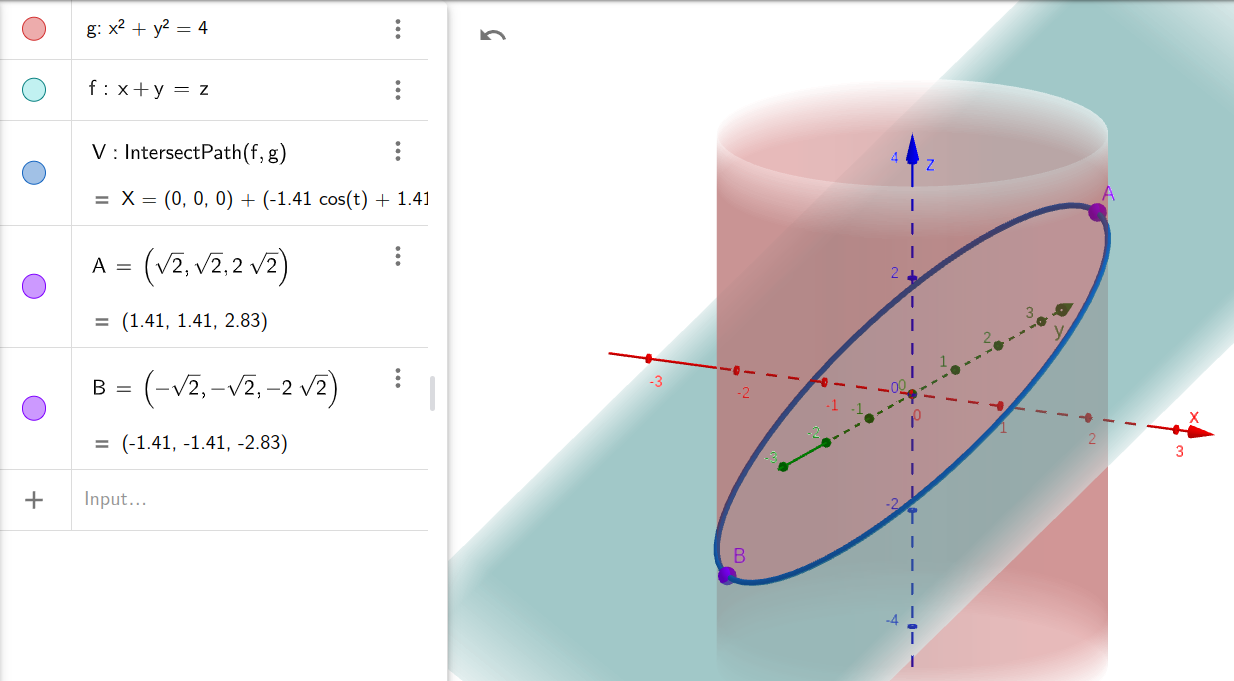
\includegraphics[width=0.8\textwidth]{esempio-ottimizzazione-con-parametrizzazione.png}
\end{center}

\pagebreak
\subsubsection{Introduzione ai moltiplicatori di Lagrange}

Come nel metodo precedente, sia \(f: A \subseteq \R^2 \to \R \) una funzione \(\in C^1(A)\); e sia il vincolo della forma \(g(x,y) = k\) con \(g(x,y) \in C^{1}(A)\)

In questo metodo imponiamo delle condizioni affinché le curve di livello della funzione coincidano in un modo particolare con la curva definita dal vincolo. Così facendo, i punti di intersezione trovati saranno punti critici candidati a essere minimi/massimi.

Introduciamo il ragionamento dietro questo metodo attraverso un esempio grafico.

Cerchiamo il massimo della funzione \(f(x,y) = xy\) ristretta sulla curva definita dalla circonferenza di raggio 1 e centro l'origine degli assi:

\[
    V = \{(x,y) \in \R^{2} \giventhat \underbrace{ x^{2}+y^{2}=1}_{g(x,y) = k} ;\  x \ge 0 ;\ y \ge 0 \}
\]

Disegniamo gli insiemi di livello della funzione \(f\):

\[
    E_c = \{(x,y) \in \R^{2} \giventhat xy = c \quad\text{per } c \in \R \}
\]

Voglio trovare il valore massimo di \(f\) in \(V\) e dunque devo trovare il valore di \(c\) per cui l'insieme di livello interseca il vincolo \(V\).

Nella seguente immagine abbiamo:
\begin{itemize}
    \item Blu: \(f(x,y) = xy\)
    \item Rosso: \(x^2 + y^2 = 1\)
    \item A{:} Intersezione
    \item Vincolo V{:} bordo nero lungo l'intersezione tra il rosso e il blu
\end{itemize}

\begin{center}
    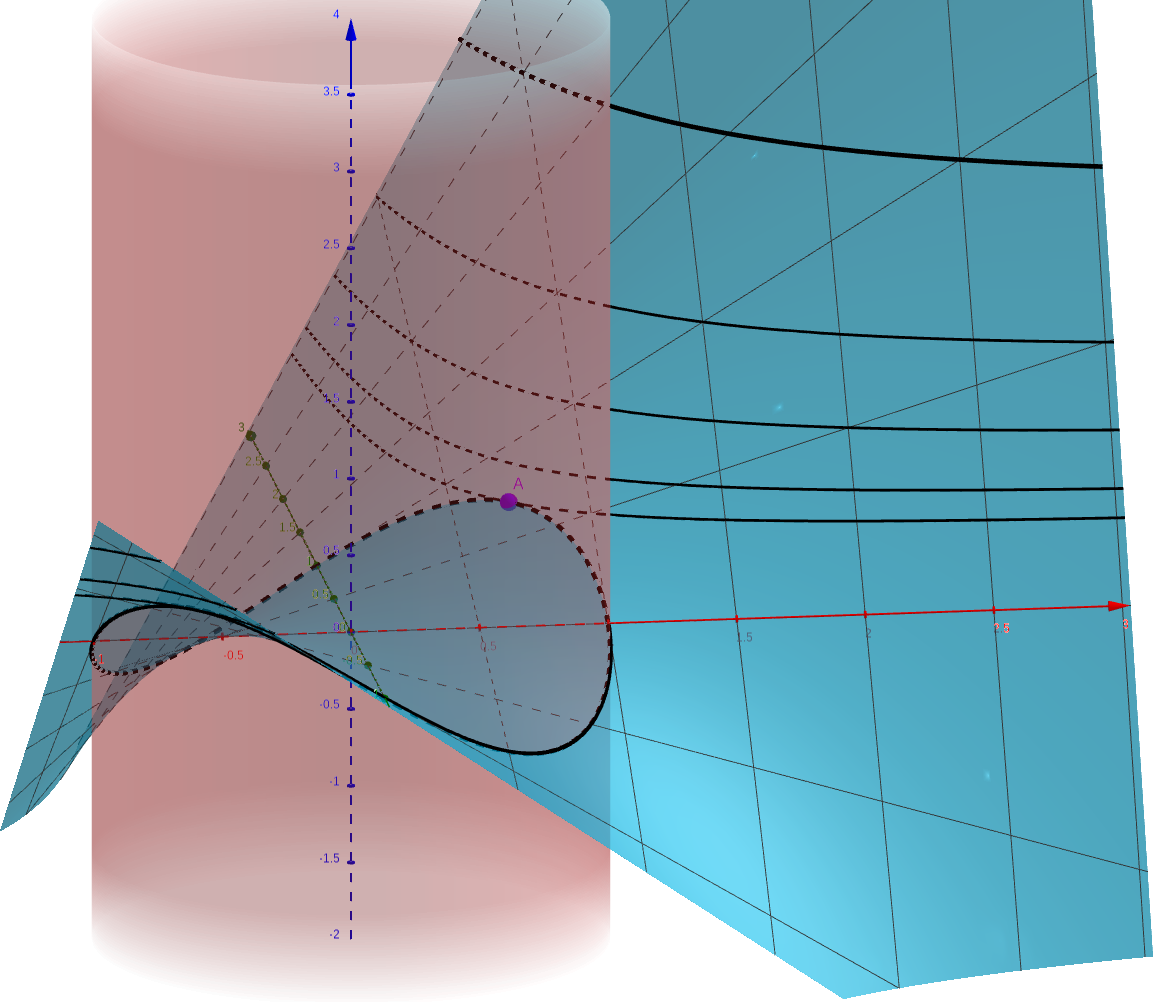
\includegraphics[width=0.6\textwidth]{esempio-ottimizzazione-con-lagrange-1.png}
\end{center}

Dal grafico possiamo osservare che nel punto viola in figura chiamato \(A\) gli insiemi \(E_c\) e \(V\) hanno la \textbf{stessa retta tangente}.

Inoltre sempre dal grafico apprendiamo che \(c = \frac{1}{2}\) e che \(A = \left(\frac{\sqrt{2}}{2}, \frac{\sqrt{2}}{2}\right)\)

Dunque, possiamo dire che la curva di livello \(xy = \frac{1}{2}\) è tangente al vincolo \(V\) in \(A\).

Riprendiamo ora il concetto della funzione composta \(h(t) = f(\gamma(t))\) come abbiamo visto nel metodo precedente; dove \(\gamma(t)\) era la curva su cui è ristretta \(f\).

Quando poco fa abbiamo parlato della tangente di \(f(x,y)\) sulla curva \(\gamma(t)\), abbiamo detto che la derivata di \(h(t)\) nel punto \(A\) è uguale a 0. Ovvero:

\[
    h'(t) = \prods{\nabla f(\gamma(t))}{\gamma'(t)} = 0
\]

Dalle nozioni di algebra lineare ricordiamo che se \(\prods{\vec{u}}{\vec{w}} = 0\) allora \(\vec{u} \perp \vec{w}\). Quindi qua possiamo dire che in tutti i punti in cui \(h'(t) = 0\), il gradiente della funzione \(f\) è \textbf{perpendicolare} al vettore della retta tangente, ovvero, è perpendicolare alla tangente della linea di livello \(E_c\).

Passiamo ora ad analizzare \(g\), la funzione del vincolo.

Per lo stesso motivo appena visto, anche il gradiente del vincolo, \(\nabla g(x_0,y_0)\), è ortogonale all'insieme di livello \(g(x,y) = k\), ovvero il vincolo stesso.

Inoltre, sappiamo che la retta tangente al vincolo ci fornisce la direzione \(\vec{v}\) in cui dobbiamo andare per rimanere sullo stesso insieme di livello (\(g(x,y) - k=0\)). Visto che \(g\) è costantemente uguale a \(k\), se allora esaminiamo la derivata direzionale:

\[
    D_{\vec{v}} g(x_0,y_0) = \langle \nabla g(x_0,y_0), \vec{v} \rangle = 0
\]

troviamo anche qui che il gradiente della \(g\) è ortogonale al vettore della retta tangente.

\begin{center}
    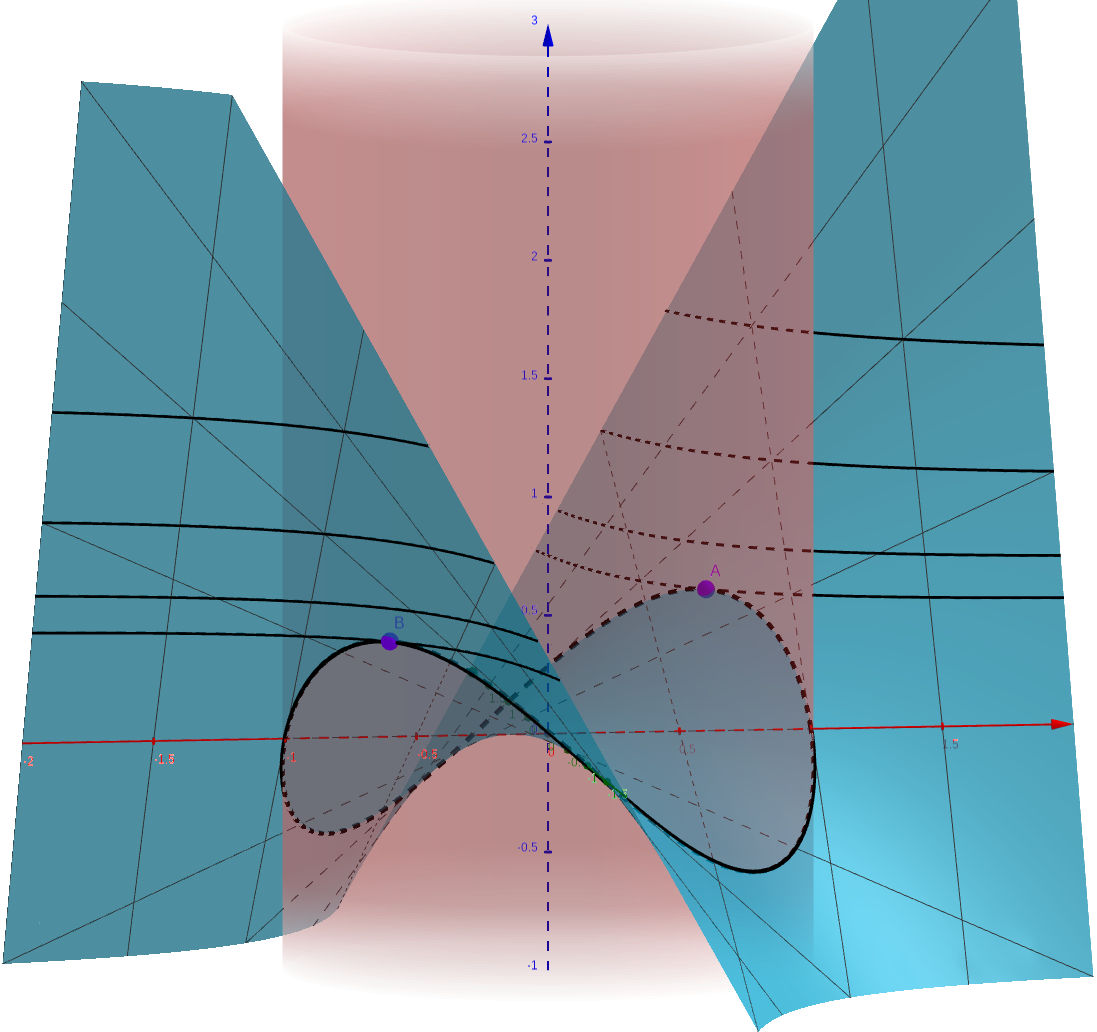
\includegraphics[width=0.6\textwidth]{esempio-ottimizzazione-con-lagrange-2.png}
\end{center}

Dunque, tutto questo ci permette di notare che i due vettori gradienti \(\nabla f(x_0,y_0)\) e \(\nabla g(x_0,y_0)\) sono di conseguenza paralleli. Ovvero \(\exists \lambda_0 \in \R \) tale che:

\[
    \nabla f(x_0,y_0) = \lambda_0 \nabla g(x_0,y_0)
\]

Questa è proprio l'osservazione dietro il metodo dei moltiplicatori di Lagrange che andiamo adesso a definire formalmente.

\pagebreak
\subsubsection{Metodo dei moltiplicatori di Lagrange}

Il seguente teorema ci dà una condizione necessaria affinché un punto sul vincolo sia di estremo.

\teorema{Moltiplicatori di Lagrange}{
    Sia \(f: A \subseteq \R^2 \to \R \) e sia \(g: A \subseteq \R^2 \to \R \), con \(A\) aperto.

    Siano inoltre \(f,g \in C^{1}(A)\).

    Sia l'insieme dei punti del vincolo \(V = \{(x,y) \in \R^2 \giventhat g(x,y) = k\} \)

    Se sono vere le seguenti condizioni:
    \begin{itemize}
        \item \((x_0,y_0)\) punto di estremo vincolato
              \hfill condizione fondamentale!
        \item \(g(x_0,y_0) = k\)
              \hfill ovvero, \((x_0,y_0)\) è in \(V\).
        \item \(\nabla g(x_0,y_0) \neq 0\)
              \hfill ovvero, la \(g\) è una \textbf{curva regolare} in \((x_0,y_0)\).
    \end{itemize}
    Allora esiste \(\lambda_0 \in \R \) tale che:
    \[
        \nabla f(x_0,y_0) = \lambda_0 \nabla g(x_0,y_0)
    \]

    I valori \(\lambda \) per cui è vera \textbf{l'equazione vettoriale} sono chiamati \textbf{moltiplicatori di Lagrange}.
}

L'equazione vettoriale sta a significare che i due vettori sono uguali in direzione e verso ma differenti in modulo (hanno lunghezze differenti). Questo succede proprio quando il vincolo e l'insieme di livello sono tangenti, ovvero solo in quel caso i gradienti sono paralleli.

Quindi, imponendo questa condizione sto effettivamente cercando il punto minimo o massimo vincolato della funzione.

Se scriviamo l'equazione vettoriale \(\nabla f(x_0,y_0) = \lambda_0 \nabla g(x_0,y_0)\) componente per componente insieme all'equazione del vincolo, ottengo un sistema di 3 equazioni:

\begin{equation*}
    \begin{cases}
        \begin{aligned}
            f_x(x,y) - \lambda g_x(x,y) & = 0 \\
            f_y(x,y) - \lambda g_y(x,y) & = 0 \\
            g(x,y)                      & = k
        \end{aligned}
    \end{cases}
\end{equation*}

le cui soluzioni sono nella forma \((x_0,y_0,\lambda_0)\).

\smallskip
Questi punti di minimo e massimo della \(f(x,y)\) ristretta al vincolo sono quindi i punti critici (gradiente nullo) della seguente funzione in tre variabili:
\[
    L(x,y,\lambda) = f(x,y) - \lambda [g(x,y) -k]
\]

detta ``\textbf{Lagrangiana}'', e se poniamo:
\[
    \nabla L(x,y,\lambda) = 0
\]

si ritrova il precedente sistema di 3 equazioni.

\smallskip
In particolare, possiamo dunque dire che le soluzioni \((x_0,y_0, \lambda_0)\) sono i punti critici di \(L\).

\pagebreak
\subsubsection{Metodo dei moltiplicatori di Lagrange {-} Esempi}

\subsubsection*{Esempio 1}

Cerchiamo gli estremi della funzione di prima \(f(x,y) = xy\) ristretta al vincolo \(g(x,y) = 1\) con \(g(x,y) = x^2+y^2\):
\[
    V= \{(x,y) \in \R^{2} \giventhat x^{2}+y^{2} = 1\}
\]

Verifichiamo innanzitutto la condizione di regolarità. Verifichiamo quindi che i punti del vincolo abbiano tutti gradiente non nullo:
\medskip
\begin{align*}
     & \nabla g(x,y) = (2x,2y)          \\
     & \nabla g(x,y) = (0,0) \iff x=y=0
\end{align*}

Il gradiente della \(g\) è nullo solo per il punto \((0,0)\), che non però in \(V\), quindi è verificata la condizione di regolarità per tutti i punti di \(V\).

Passiamo ora all'equazione vettoriale:
\medskip
\begin{equation*}
    \begin{cases}
        f_x(x,y) - \lambda g_x(x,y) = 0 \\
        f_y(x,y) - \lambda g_y(x,y) = 0 \\
        g(x,y) = k
    \end{cases}
\end{equation*}
\smallskip
\begin{equation*}
    \begin{split}
        & \implies
        \begin{cases}
            y -2 \lambda x= 0  \\
            x -2 \lambda y = 0 \\
            x^{2}+ y^{2}= 1
        \end{cases}
        \,\xrightarrow[]{x \ne 0}
        \begin{cases}
            \lambda= \frac{y}{2x}  \\
            x-2( \frac{y}{2x})y= 0 \\
            x^{2}+ y^{2}= 1
        \end{cases}
        \,\implies
        \begin{cases}
            \lambda= \frac{y}{2x} \\
            x^{2}-y^{2}= 0        \\
            x^{2}+ y^{2}= 1
        \end{cases} \\
        & \implies
        \begin{cases}
            \lambda= \frac{y}{2x} \\
            y= \pm x              \\
            x^{2}+ y^{2}= 1
        \end{cases}
        \,\implies
        \begin{cases}
            x = \pm \frac{1}{\sqrt{2}} \\
            y= \pm x                   \\
        \end{cases}
    \end{split}
\end{equation*}

Nei primi passaggi è stato possibile dividere per \(x\) in quanto in \(V\) tutti i punti hanno la \(x \ne 0\).

Senza trascrivere i moltiplicatori di Lagrange (\(\lambda= \frac{y}{2x}\)), abbiamo quindi questi estremi vincolati:
\medskip
\begin{align*}
    A=\left( -\frac{1}{\sqrt{2}}, -\frac{1}{\sqrt{2}} \right)
     &  &
    B=\left(  \frac{1}{\sqrt{2}},  \frac{1}{\sqrt{2}} \right)
     &  &
    C=\left( -\frac{1}{\sqrt{2}},  \frac{1}{\sqrt{2}} \right)
     &  &
    D=\left(  \frac{1}{\sqrt{2}}, -\frac{1}{\sqrt{2}} \right)
\end{align*}

Calcoliamo la funzione in questi punti:
\medskip
\begin{align*}
    f(A) = \frac{1}{2} &  & f(B) = \frac{1}{2} &  & f(C) = -\frac{1}{2} &  & f(D) = - \frac{1}{2}
\end{align*}

e dunque \(A,B\) sono massimi e \(C,D\) sono minimi:

Infatti, la curva di livello:
\[
    E_{ 1/2} = \{(x,y) \in \R^{2} \giventhat xy = 1/2\}
\]

è tangente al vincolo \(V\) nei punti \(A\) e \(B\); e la curva di livello:
\[
    E_{ -1/2} = \{(x,y) \in \R^{2} \giventhat xy = -1/2\}
\]

è tangente al vincolo \(V\) nei punti \(C\) e \(D\).

\pagebreak
\subsubsection{Esercizi}

\subsubsection*{Esercizio 1}

Utilizzando entrambi i metodi di ottimizzazione, determinare gli estremi di \(f(x,y) = 3x + 4y +1\) vincolati all'ellisse di equazione \({\left(\frac{x}{2}\right)}^{2}+ {\left(\frac{y}{3}\right)}^{2}=1\).

\[
    V = \left\{(x,y) \in \R^{2} \giventhat[\bigg] {\left(\frac{x}{2}\right)}^{2}+ {\left(\frac{y}{3}\right)}^{2}-1=0\right\}
\]

Per semplificare la comprensione dell'esempio, cominciamo immaginandoci il grafico.
\begin{itemize}
    \item la funzione \(f\) è il piano di colore rosso;
    \item l'ellisse del vincolo, ovvero \(g\), è rappresentata sia come curva del livello \(z=0\) che come intersezione tra i punti della funzione e i punti del vincolo;
    \item I punti di minimo e massimo sono rispettivamente i punti fucsia \(P_1\) e \(P_2\).
\end{itemize}
\begin{center}
    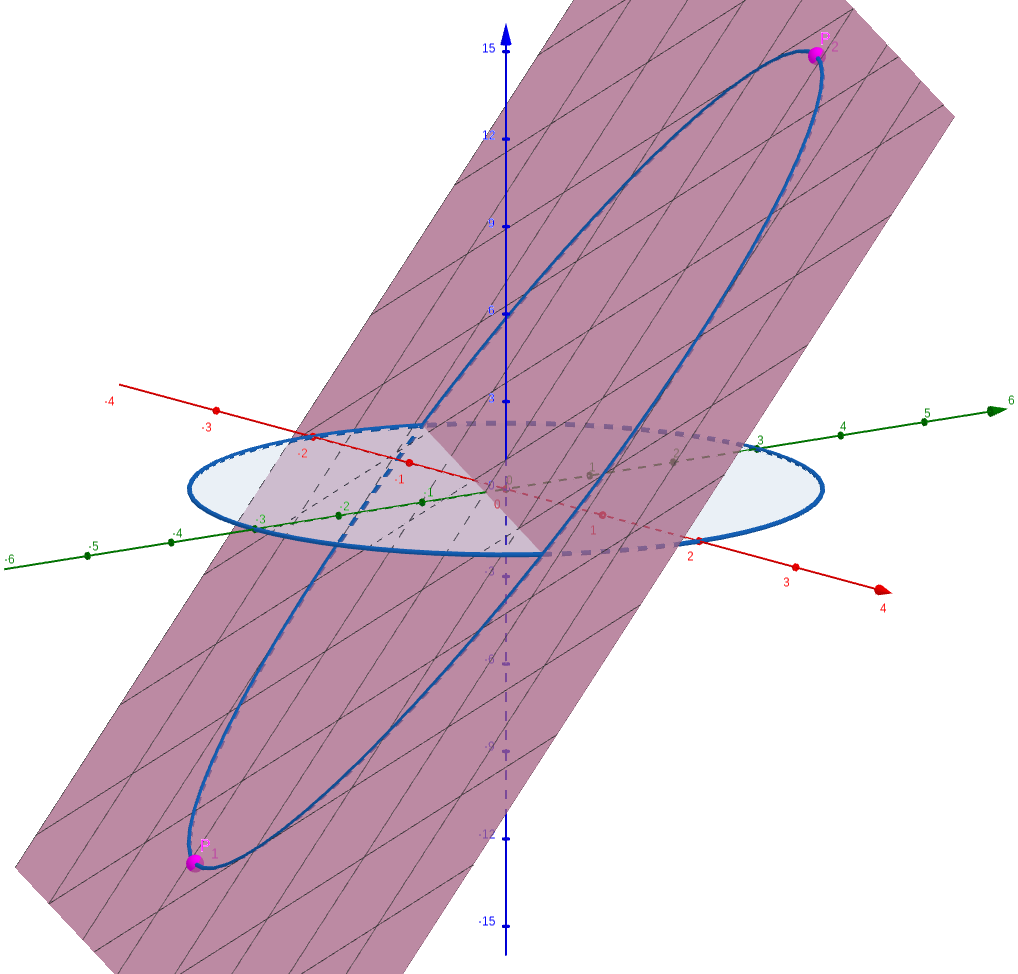
\includegraphics[width=0.9\textwidth]{esercizio-2-ottimizzazione.png}
\end{center}

\filbreak{}
\subsubsection*{Metodo di parametrizzazione}

Determinare gli estremi di \(f(x,y) = 3x + 4y +1\) vincolati all'ellisse di equazione \({\left(\frac{x}{2}\right)}^{2}+ {\left(\frac{y}{3}\right)}^{2}=1\).

Parametrizzo il vincolo come sostegno della curva piana regolare:
\begin{align*}
     & \gamma: [0,2\pi] \to \R^2 \\[2mm]
     & \gamma: \begin{cases}
                   x(t) = 2 \cos(t) \\
                   y(t) = 3 \sin(t)
               \end{cases}
\end{align*}
Trovi i punti critici:

\vspace{3mm}
\(\nabla f(x,y) = (3,4)\)

\(\nabla f(\gamma(t)) = (3,4)\)

\(h(t) = f(\gamma(t)) = 6 \cos(t) + 12 \sin(t) + 1\)

\(h'(t) = \prods{\nabla f(\gamma(t))}{\gamma'(t)} = \prods{(3,4)}{(-2\sin(t),3\cos(t))} = -6 \sin(t) + 12 \cos(t)\)
\vspace{3mm}

I punti critici quindi soddisfano questa equazione:
\[
    h'(t) = 0 \iff -6 \sin(t) + 12 \cos(t) = 0 \implies 2 \cos(t) - \sin(t) = 0
\]
Scrivo in funzione di una sola variabile, la \(y\):
\[
    2 \cos(t) = \sin(t) \iff x = \frac{1}{3}y
\]

Adesso sostituisco quello che ho trovato nella \(g(x,y)\):

\[
    \left[ \frac{1}{4} \cdot {\left(\frac{y}{3}\right)}^{2} \right] + \left[ \frac{y^{2}}{9} \right] = 1
\]

\[
    \frac{y^{2}}{36} + \frac{y^{2}}{9} = 1
    \implies
    \frac{5}{36} y^{2} = 1
    \implies
    \begin{cases*}
        y = \pm \frac{6}{\sqrt{5}} \\
        x = \frac{1}{3}y
    \end{cases*}
\]

Dunque abbiamo ottenuto i punti:

\[
    P_1=\begin{cases}
        x= - \frac{2}{\sqrt{5}} \\
        y = -\frac{6}{\sqrt{5}}
    \end{cases}
    \implies
    f(P_1) = -6 \sqrt{5} + 1
    \implies
    \text{minimo}
\]

\[
    P_2=\begin{cases}
        x=  \frac{2}{\sqrt{5}} \\
        y = \frac{6}{\sqrt{5}}
    \end{cases}
    \implies
    f(P_2) = 6 \sqrt{5} + 1
    \implies
    \text{massimo}
\]

\filbreak{}
\subsubsection*{Metodo dei moltiplicatori di Lagrange}

Determinare gli estremi di \(f(x,y) = 3x + 4y +1\) vincolati all'ellisse di equazione \({\left(\frac{x}{2}\right)}^{2}+ {\left(\frac{y}{3}\right)}^{2}=1\).

Verifico la condizione di regolarità, ovvero, verifico che i punti del vincolo abbiano tutti gradiente non nullo:

\[
    \nabla g(x,y) = \left( \frac{x}{2}, \frac{2}{9}y \right) = (0,0) \iff x=y = 0
\]

dato che \((0,0) \notin V\) posso applicare il metodo dei moltiplicatori di Lagrange.

Trovo quindi i punti critici della Lagrangiana \(L(x,y,\lambda)\), ovvero pongo \(\nabla L(x,y,\lambda) = 0\):

\[
    \begin{cases*}
        f_x - \lambda g_x = 0 \\
        f_y - \lambda g_y = 0 \\
        g(x,y) = k            \\
    \end{cases*}
    \implies
    \begin{cases*}
        3- \lambda \frac{1}{2}x = 0   \\
        4 - \lambda \frac{2}{9} y = 0 \\
        {(\frac{x}{2})}^{2}+{(\frac{y}{3})}^{2}=1
    \end{cases*}
    \implies
    \begin{cases*}
        \lambda = \frac{6}{x}                               \\
        4 - \left( \frac{6}{x} \right)\cdot\frac{2}{9}y = 0 \\
        \frac{1}{4}x^2 + \frac{1}{9}y^2 = 1
    \end{cases*}
    \implies
    \begin{cases*}
        \lambda = \frac{6}{x} \\
        y = 3x                \\
        x = \pm \frac{2}{\sqrt{5}}
    \end{cases*}
\]

Abbiamo quindi, come in precedenza, i due punti:

\[
    P_1=\begin{cases}
        x= - \frac{2}{\sqrt{5}} \\
        y = -\frac{6}{\sqrt{5}}
    \end{cases}
    \implies
    f(P_1) = -6 \sqrt{5} + 1
    \implies
    \text{minimo}
\]

\[
    P_2=\begin{cases}
        x=  \frac{2}{\sqrt{5}} \\
        y = \frac{6}{\sqrt{5}}
    \end{cases}
    \implies
    f(P_2) = 6 \sqrt{5} + 1
    \implies
    \text{massimo}
\]


\end{document}
